\documentclass[12pt]{article}
\PassOptionsToPackage{hyphens}{url}

\usepackage{sbc-template}
\usepackage{graphicx,url}
\usepackage[utf8]{inputenc}
\usepackage[brazil]{babel}
\usepackage{booktabs}
\usepackage{multirow}
\usepackage{tabularx}
\usepackage{array}
\newcolumntype{P}[1]{>{\raggedright\hyphenpenalty=10000\exhyphenpenalty=10000\arraybackslash}p{#1}}
\usepackage{float}
\usepackage{amsmath}
\newcolumntype{Y}{>{\raggedright\arraybackslash}X}

\sloppy

\title{Uso de Modelos de Linguagem na Implementação da Pirâmide de
Testes: Um Estudo de Caso em uma Aplicação Móvel}

\author{Marcos Leite Bezerra Neto\inst{1}, Cleyton Magalhães\inst{1}}

\address{Departamento de Estatística e Informática\\
  Universidade Federal Rural de Pernambuco (UFRPE)\\
  Recife -- PE -- Brasil
  \email{marcos.leiten@ufrpe.br, cleyton.vanut@ufrpe.br}
}

\begin{document}

\maketitle

\begin{abstract}
Implementing tests across every level of the test pyramid is labor-intensive
and tends to leave coverage uneven. This work asks whether large language
models, guided by prompt-engineering strategies, can implement a complete test
pyramid for a real mobile application, and whether the tests they produce
actually protect the system. A case study on Sintonize (Flutter + Firebase)
ran 156 rounds under a fixed protocol: three strategies (zero-shot, few-shot,
chain-of-thought) $\times$ two models accessed through their web interfaces
(ChatGPT and Gemini) $\times$ four levels (unit, widget, integration and
end-to-end on an Android emulator with the Firebase Emulator Suite), with nine
planted defects as an oracle and a two-way repair template under which the
model classifies each failure as a test error or a suspected application
defect. Executability and defect detection were measured separately. Both
models implement the pyramid (93\% pass rate on clean targets), but the
resulting tests capture the defect in only 5 and 7 of the 27 exposures per
model (nine defects $\times$ three strategies; two ChatGPT cells without
data); of the remainder, most fix the defect by assertion as the expected
behavior --- with a warning in prose (15 cases) or silently, the
\emph{canonization} (7) --- or never exercise it (14). Canonization arises at
generation time, and the repair loop, effective at preventing the model from
weakening assertions, does not reach it. Prompt strategy does not order the
results; defect type and the material supplied in the prompt do. The two
models exhibit pyramids of different shape, with neither dominating. The study
also exposed five real defects in the application and is reported following
the guidelines of Baltes et al. (2026), with a complete replication package.
\end{abstract}

\noindent\textbf{Keywords:} Large Language Models; Automated Test Generation; Test Pyramid; Prompt Engineering; Flutter; Planted Defects.

\begin{resumo}
Implementar testes em todos os níveis da pirâmide de testes é trabalhoso e
tende a deixar a cobertura desigual. Este trabalho pergunta se modelos de
linguagem de grande escala, guiados por estratégias de engenharia de
\textit{prompt}, conseguem implementar uma pirâmide de testes completa para
uma aplicação móvel real, e se os testes que produzem de fato protegem o
sistema. Um estudo de caso no Sintonize (Flutter + Firebase) executou 156
rodadas sob um protocolo fixo: três estratégias (\textit{zero-shot},
\textit{few-shot}, \textit{chain-of-thought}) $\times$ dois modelos acessados
pela interface \textit{web} (ChatGPT e Gemini) $\times$ quatro níveis
(unitário, \textit{widget}, integração e \textit{end-to-end} em emulador
Android com o Firebase Emulator Suite), com nove defeitos plantados como
oráculo e um \textit{template} de reparo em duas vias, sob o qual o modelo
classifica cada falha como erro do teste ou suspeita de defeito da aplicação.
Executabilidade e detecção de defeitos foram medidas separadamente. Os dois
modelos implementam a pirâmide (93\% de aprovação nos alvos limpos), mas os
testes resultantes capturam o defeito em apenas 5 e 7 das 27 exposições por
modelo (nove defeitos $\times$ três estratégias; duas do ChatGPT sem dado); do
restante, a maior parte fixa o defeito por asserção como comportamento
esperado --- com aviso em prosa (15 casos) ou em silêncio, a
\emph{canonização} (7) --- ou nem chega a exercitá-lo (14). A canonização
nasce na geração, e o ciclo de reparo, eficaz em impedir que o modelo
enfraqueça asserções, não a alcança. A estratégia de
\textit{prompt} não ordena os resultados; o tipo de defeito e o material
fornecido no \textit{prompt} ordenam. Os dois modelos exibem pirâmides de
forma diferente, sem que um domine o outro. O estudo expôs ainda cinco
defeitos reais da aplicação e é relatado segundo as diretrizes de Baltes et
al. (2026), com pacote de replicação completo.
\end{resumo}

\noindent\textbf{Palavras-chave:} Modelos de Linguagem de Grande Escala; Geração Automática de Testes; Pirâmide de Testes; Engenharia de Prompt; Flutter; Defeitos Plantados.

% ============================================================
\section{Introdução}
\label{sec:introducao}

A qualidade de software tornou-se um fator determinante para o sucesso de
organizações em praticamente todos os setores da economia. Com a crescente
dependência de sistemas digitais para operações críticas, falhas de software
deixaram de ser inconvenientes técnicos e passaram a representar riscos
financeiros, operacionais e reputacionais. Segundo o \textit{Consortium for
Information and Software Quality} (CISQ), o custo da baixa qualidade de
software nos Estados Unidos alcançou 2,41 trilhões de dólares em
2022~\cite{cisq2022}, e estudos clássicos mostram que o custo de corrigir um
defeito cresce de forma acentuada quanto mais tarde ele é
identificado~\cite{boehm2001}. Nesse cenário, os testes de software ocupam
papel central na garantia da qualidade.

Para estruturar a prática de testes, a indústria adotou amplamente o modelo
da pirâmide de testes, proposto por Cohn~\cite{cohn2009} e refinado por
Vocke~\cite{vocke2018}: camadas de quantidade decrescente da base ao topo ---
unitário, integração, \textit{end-to-end} (E2E) --- que equilibram velocidade de
\textit{feedback} e custo de manutenção (Seção~\ref{subsec:piramide}).
Implementar a pirâmide, porém, é trabalhoso: a criação manual de casos de
teste em cada nível consome tempo, é suscetível ao viés de quem escreve e
resulta com frequência em cobertura desigual~\cite{cohn2009}.

Os Modelos de Linguagem de Grande Escala (\textit{Large Language Models} ---
LLMs) surgiram como candidatos naturais a reduzir esse esforço. Estudos
recentes documentam seu uso na geração de casos de teste unitários,
reprodução de defeitos, escrita de \textit{scripts} de automação e criação de
oráculos~\cite{wang2024survey,santana2025software}. Em um estudo com 15
profissionais, Santana et al.~\cite{santana2025software} observaram que essa
adoção segue um processo iterativo e reflexivo --- definir o objetivo,
aplicar estratégias de engenharia de \textit{prompt}, refinar, avaliar as
saídas --- sempre mediado por supervisão humana, por causa de alucinações e
raciocínio inconsistente, e ainda sem padrões estabelecidos para integrar
essas ferramentas ao ciclo de testes.

A pesquisa sobre geração de testes com LLMs distribui-se de forma desigual
pela pirâmide. Ferramentas como ChatUniTest~\cite{chen2024chatunitest}
concentram-se no nível unitário, onde os resultados são mais promissores;
trabalhos conceituais, como o de Desai et al.~\cite{desai2025testpyramid},
propõem que a Inteligência Artificial pode potencializar todas as camadas,
mas reconhecem que a evidência empírica é escassa. E há uma segunda lacuna,
menos visível: a maior parte dos estudos mede a qualidade dos testes gerados
pela \emph{taxa de aprovação} --- a proporção de testes que compilam e passam
---, uma métrica que não distingue um teste correto de um teste que fixou um
defeito do sistema como comportamento esperado. Um conjunto de testes gerado
automaticamente pode estar inteiramente verde e proteger contra muito pouco.
Separar essas duas coisas exige um oráculo: defeitos conhecidos, contra os
quais se possa perguntar se o teste gerado falha.

Há, por fim, um problema de método que atravessa toda essa literatura. Baltes
et al.~\cite{baltes2026guidelines} mostram que estudos empíricos com LLMs em
Engenharia de Software são difíceis de reproduzir --- de 18 artigos de
conferências de primeira linha que usaram modelos da OpenAI e publicaram
artefatos, nenhum teve seus resultados reproduzidos --- por não determinismo,
modelos comerciais que mudam sem aviso sob o mesmo nome e relato incompleto de
\textit{prompts}, versões e configurações. Os autores propõem oito diretrizes
de desenho e relato, que este trabalho adota.

Diante dessas lacunas, este trabalho investiga o uso de LLMs na implementação
de uma pirâmide de testes completa, por meio de um estudo de caso no
Sintonize, uma aplicação móvel de recomendação musical desenvolvida em
Flutter~\cite{flutter} com \textit{backend} Firebase. Testes unitários, de
\textit{widget}, de integração e E2E foram gerados por dois
modelos acessados pela interface \textit{web} --- ChatGPT e Gemini ---, sob
três estratégias de engenharia de \textit{prompt} --- \textit{zero-shot},
\textit{few-shot} e \textit{chain-of-thought} --- e um protocolo fixo de
rodadas com ciclo de reparo. Nove defeitos foram plantados na aplicação, um
CRASH --- exceção não tratada, que interrompe o fluxo --- e um SILENT ---
resultado errado sem nenhum erro visível --- por nível (três no E2E), de
modo que cada teste gerado pudesse ser avaliado em
duas dimensões independentes: se \emph{executa} e se \emph{detecta}. Nos
três níveis inferiores o defeito estava no código colado no \textit{prompt};
no E2E o \textit{prompt} era limpo e o teste rodava contra a versão com
defeito, no aplicativo real em emulador Android com o pacote
\texttt{integration\_test} e o Firebase Emulator Suite.

O objetivo geral é caracterizar benefícios, dificuldades e limites do uso de
LLMs na implementação da pirâmide de testes. Os objetivos específicos são:
(i)~comparar as três estratégias de \textit{prompt} e os dois modelos em cada
nível, em executabilidade e em detecção; (ii)~identificar as dificuldades
específicas de cada nível e as suas causas; (iii)~caracterizar os modos de
falha dos testes gerados diante de defeitos conhecidos, em particular a
canonização; (iv)~catalogar os defeitos reais da aplicação expostos pelo
processo; e (v)~entregar um protocolo e um pacote de replicação conformes às
diretrizes de Baltes et al.~\cite{baltes2026guidelines}.

A questão de pesquisa é: \textit{em que medida modelos de linguagem, guiados
por estratégias de engenharia de \textit{prompt}, implementam uma pirâmide de
testes que de fato protege uma aplicação móvel real, e quais são os desafios
encontrados em cada nível?} A delimitação importa: trata-se de um estudo de
caso em um único aplicativo, com dois modelos acessados nas condições em que o
desenvolvedor sem acesso à API os encontra (sessão gratuita ou padrão), uma
rodada por combinação de alvo, estratégia e modelo, e codificação de
detecção feita por um único avaliador. Os resultados descrevem padrões
nesse contexto e não autorizam inferência estatística; as ameaças à validade
são tratadas na Seção~\ref{subsec:ameacas}.

O restante do texto está organizado em seis seções e três apêndices. A
Seção~\ref{sec:referencial} apresenta o referencial teórico: a pirâmide, os
níveis de teste, os modelos de linguagem na geração de testes, as estratégias
de \textit{prompt} e os defeitos plantados como oráculo. A
Seção~\ref{sec:relacionados} discute os trabalhos relacionados e posiciona a
lacuna. A Seção~\ref{sec:metodologia} descreve o desenho, o objeto de estudo,
os defeitos plantados, o protocolo de rodada, as condições de sessão e as
métricas. A Seção~\ref{sec:resultados} apresenta os resultados pela pirâmide:
alvos limpos, detecção por defeito, autoclassificação, defeitos reais,
análise de erro, cobertura e custo. A Seção~\ref{sec:discussao} responde à
questão de pesquisa, interpreta os resultados e discute as ameaças à
validade. A Seção~\ref{sec:conclusao} retoma os objetivos, as contribuições,
as limitações e os trabalhos futuros. Os apêndices reúnem os \textit{prompts}
representativos, as limitações de testabilidade da aplicação e a lista
completa de desvios e ocorrências.

% ============================================================
\section{Referencial Teórico}
\label{sec:referencial}

Esta seção apresenta os conceitos que fundamentam o trabalho: o modelo da
pirâmide de testes e sua organização em níveis, os tipos de teste que
compõem cada camada, o uso de modelos de linguagem na geração de testes e as
estratégias de engenharia de \textit{prompt} comparadas no estudo.

\subsection{A Pirâmide de Testes}
\label{subsec:piramide}

A pirâmide de testes é um modelo conceitual proposto por Mike
Cohn~\cite{cohn2009} para orientar a distribuição de testes automatizados em
uma suíte de testes. O modelo organiza os testes em camadas dispostas em
formato de pirâmide, nas quais a quantidade de testes diminui conforme se
sobe da base ao topo. A lógica subjacente é econômica: testes nas camadas
inferiores são rápidos, determinísticos e baratos de manter, enquanto testes
nas camadas superiores são mais lentos, frágeis e custosos, devendo portanto
ser usados de forma mais seletiva~\cite{vocke2018}. O modelo busca, assim,
equilibrar velocidade de \textit{feedback}, custo de manutenção e
abrangência da validação.

Em sua formulação original, a pirâmide possui três camadas: testes unitários
na base, testes de serviço (ou integração) no meio e testes de interface ou
\textit{end-to-end} (E2E) no topo~\cite{cohn2009}. Trabalhos posteriores,
contudo, propõem versões mais granulares. Desai et al.~\cite{desai2025testpyramid}, por
exemplo, operam sobre uma pirâmide de cinco camadas --- unitário,
componente, integração, UI/API e exploratório/manual ---, argumentando que
essa granularidade reflete melhor as metodologias de teste empregadas na
indústria e na academia atualmente. Essa distinção é relevante para o
presente trabalho, pois o ecossistema utilizado no estudo de caso, o Flutter,
oferece uma camada de testes de \textit{widget} que se posiciona entre os
níveis unitário e de integração, alinhando-se a essas formulações mais
granulares do modelo.

\subsection{Níveis de Teste}
\label{subsec:niveis}

Cada camada da pirâmide corresponde a um tipo de teste com escopo e propósito
distintos. Os \textbf{testes unitários} ocupam a base e verificam o
comportamento de unidades isoladas de código --- tipicamente uma função ou
método --- de forma rápida e independente, frequentemente recorrendo a
\textit{stubs} ou \textit{mocks} para isolar dependências
externas~\cite{desai2025testpyramid}. Por seu baixo custo e rápida execução,
fornecem o ciclo de \textit{feedback} mais ágil e são considerados
candidatos ideais à automação.

Os \textbf{testes de integração} situam-se em uma camada intermediária e
validam a interação entre múltiplos componentes ou serviços, verificando se
diferentes módulos se comunicam e funcionam corretamente em conjunto.
Diferentemente dos testes unitários, geralmente não isolam dependências por
meio de \textit{mocks}, sendo executados em ambientes mais próximos do
real~\cite{desai2025testpyramid}. Já os \textbf{testes
\textit{end-to-end} (E2E)} ocupam o topo da pirâmide e avaliam o sistema sob
a perspectiva do usuário final, simulando fluxos completos de interação por
meio da interface. São os testes de maior escopo e menor isolamento,
apresentando o ciclo de \textit{feedback} mais lento e o maior custo de
manutenção.

No contexto do Flutter, \textit{framework} utilizado no estudo de caso, esses
níveis materializam-se em três tipos de teste nativos. Os \textit{unit tests}
correspondem aos testes unitários; os \textit{widget tests} verificam
componentes de interface de forma isolada, sem dispositivo ou emulador,
ocupando uma posição intermediária entre o teste unitário e o de integração;
e os \textit{integration tests}, construídos com o pacote
\texttt{integration\_test}, executam a aplicação real em um dispositivo ou
emulador, dirigindo a interface a partir da tela de boas-vindas. Neste trabalho, o
nível que o Flutter chama de ``integração'' é usado em dois graus: testes de
fluxo entre telas com dublês de Firebase, executados por \texttt{flutter
test} sem dispositivo (aqui chamados de \textbf{integração}), e testes do
aplicativo completo em emulador Android contra o Firebase Emulator Suite ---
serviços locais de Authentication e Firestore que substituem o
\textit{backend} de produção com o mesmo protocolo --- (aqui chamados de
\textbf{E2E}). A distinção importa porque os obstáculos de cada grau são
diferentes: o primeiro depende de isolar dependências com dublês; o segundo,
de infraestrutura, sincronização com a interface e dados semeados.

\subsection{Modelos de Linguagem na Geração de Testes}
\label{subsec:llms}

Modelos de Linguagem de Grande Escala (\textit{Large Language Models} ---
LLMs) são sistemas de inteligência artificial treinados sobre grandes volumes
de texto e código, capazes de gerar linguagem natural e artefatos de software
estruturados a partir de uma entrada ou \textit{prompt}~\cite{wang2024survey}.
Sua capacidade de compreender linguagem natural e produzir código os tornou
candidatos naturais para a automação de tarefas na engenharia de software,
incluindo a geração de testes.

No domínio de testes, os LLMs vêm sendo aplicados a tarefas como geração de
casos de teste unitários, reprodução de defeitos, escrita de \textit{scripts}
de automação, criação de oráculos e documentação~\cite{wang2024survey,
santana2025software}. Ferramentas como o ChatUniTest~\cite{chen2024chatunitest}
demonstram a viabilidade da abordagem no nível unitário, alcançando cobertura
superior à de técnicas tradicionais baseadas em algoritmos evolutivos. Um
desafio recorrente, no entanto, é a natureza não determinística desses
modelos, que pode produzir saídas sintaticamente corretas mas semanticamente
inadequadas, além de alucinações e raciocínio inconsistente~\cite{santana2025software}.
Para mitigar esse problema, a literatura aponta o uso de ciclos iterativos
de validação e reparo (\textit{repair loops}), nos quais a saída do modelo é
executada e os erros são realimentados ao modelo até que se obtenha um
resultado satisfatório ou se atinja um limite de tentativas; esse padrão foi
observado entre profissionais de teste por Santana et
al.~\cite{santana2025software} e é o núcleo de ferramentas como o
TestPilot~\cite{schafer2024testpilot}. O ciclo de reparo tem, porém, um
efeito colateral que a avaliação por taxa de aprovação não revela: pressionado
a fazer o teste passar, o modelo pode ajustar a asserção ao comportamento
observado, e um comportamento observado pode ser um defeito. O teste
resultante passa, parece correto e documenta o defeito como especificação.
Avaliar a geração de testes com LLMs exige, portanto, distinguir dois
construtos --- se o teste \emph{executa} e se o teste \emph{protege} ---, o
que motiva o uso de defeitos conhecidos como oráculo, tratado na
Seção~\ref{subsec:oraculo}. Baltes et al.~\cite{baltes2026guidelines}
sistematizam essa e outras exigências de desenho e relato para estudos
empíricos com LLMs em Engenharia de Software, em oito diretrizes que este
trabalho segue.

\subsection{Engenharia de Prompt}
\label{subsec:prompt}

A engenharia de \textit{prompt} consiste no processo de elaborar as entradas
fornecidas a um LLM de modo a guiar seu comportamento e obter as saídas
desejadas. Tornou-se a estratégia dominante para a geração de testes com
LLMs, e a forma como o \textit{prompt} é construído influencia diretamente a
qualidade dos artefatos gerados~\cite{wang2024survey}. Neste trabalho, três
estratégias de engenharia de \textit{prompt} são comparadas, escolhidas por
representarem uma progressão crescente no grau de orientação fornecido ao
modelo:

\begin{itemize}
  \item \textbf{\textit{Zero-shot}:} o modelo recebe apenas a descrição da
  tarefa, sem exemplos de saída esperada~\cite{kojima2022}. Constitui o
  cenário de menor esforço de \textit{prompting} e serve como linha de base para
  comparação.

  \item \textbf{\textit{Few-shot}:} o \textit{prompt} inclui alguns exemplos
  de testes corretos, que servem de referência para o
  modelo~\cite{brown2020}. A estratégia avalia o ganho obtido ao fornecer
  exemplos que demonstram o padrão esperado.

  \item \textbf{\textit{Chain-of-thought} (COT):} solicita-se que o modelo
  explicite seu raciocínio passo a passo antes de produzir o resultado
  final~\cite{wei2022}. A estratégia avalia o efeito de induzir o
  raciocínio explícito sobre a qualidade dos testes gerados.
\end{itemize}

A comparação entre essas três estratégias, aplicadas de forma sistemática aos
diferentes níveis da pirâmide, constitui o eixo central da investigação
conduzida neste trabalho.

\subsection{Defeitos Plantados como Oráculo}
\label{subsec:oraculo}

Um teste automatizado só tem valor se falhar quando o sistema está errado.
Medir essa propriedade exige saber onde o sistema está errado, e a técnica
clássica para isso é introduzir defeitos conhecidos e verificar se a suíte
os detecta --- a ideia que fundamenta o teste de mutação, no qual pequenas
alterações sintáticas (mutantes) são aplicadas ao código e um mutante é
considerado ``morto'' quando ao menos um teste falha~\cite{jia2011mutation}.
A proporção de mutantes mortos (\textit{mutation score}) é uma medida da
capacidade de detecção da suíte, independente da sua taxa de aprovação e da
sua cobertura.

Este trabalho adota uma forma dirigida dessa ideia: em vez de mutantes
gerados automaticamente em grande número, poucos defeitos
\textbf{plantados} manualmente, cada um uma alteração de uma linha, plausível
como erro de programação e observável por um teste do nível correspondente da
pirâmide. Os defeitos são de dois tipos. No tipo \textbf{CRASH}, o
comportamento errado se manifesta como exceção não tratada; no tipo
\textbf{SILENT}, o sistema continua funcionando com um resultado errado
(mensagem trocada, valor fixo, navegação para a tela indevida). A
distinção é relevante para modelos de linguagem porque os dois tipos se
comportam de forma diferente quando o teste não os espera: uma exceção
derruba o teste por si só, sem depender de asserção; um valor errado só é
percebido se alguma asserção o compara ao valor certo. Quando o modelo vê o
código com defeito, porém, os dois podem ser fixados como esperado --- um
\texttt{expect(\ldots, throwsA(\ldots))} canoniza uma exceção tanto quanto
um \texttt{expect(x, 'errado')} canoniza um valor.

Plantar defeitos tem um preço e uma fraqueza. O preço é operacional: é
preciso manter duas versões do aplicativo, limpa e com defeito, e executar
rodadas nas duas, o que dobra o trabalho. A fraqueza é que os defeitos são
escolhidos pelo pesquisador e podem não se parecer com os defeitos que o
sistema realmente tem; por isso, os defeitos reais que aparecem durante o
estudo sem terem sido plantados servem de contraprova de que o oráculo não é
artificial.

Há ainda uma escolha de desenho. O modelo pode receber o código \textbf{com}
o defeito --- \emph{defeito visível} ---, e então se mede se ele percebe que
algo está errado e escreve um teste que falha, ou se fixa o erro como regra.
Ou pode receber o código \textbf{limpo} enquanto o teste gerado roda contra
a versão com defeito --- \emph{defeito oculto}, o esquema do teste de
mutação ---, e então se mede se o teste é sensível o bastante para quebrar
quando o comportamento muda. Este trabalho usa os dois regimes, um por fase
(Seção~\ref{subsec:alvos}). Em ambos, o oráculo permite dar uma nota a cada
teste gerado, do melhor caso (falhou por causa do defeito e foi mantido
assim) ao pior (nunca chegou perto do defeito); é essa nota, definida na
Seção~\ref{subsec:metricas}, que separa a detecção da executabilidade.

% ============================================================
% ============================================================
% TRABALHOS RELACIONADOS — reescrita para o estudo revisado
% Substitui a Seção 3 do main.tex. Mantém as citações existentes
% (wang2024survey, celik2025review, desai2025testpyramid, plein2023bugreports,
% hasan2025highlevel, fonseca2025atomic, cohn2009) e acrescenta
% schafer2024testpilot, liu2024gptdroid, yoon2024droidagent, liu2023qtypist,
% medeiros2026acessibilidade, baltes2026guidelines (ver bib_adicoes.bib).
% ============================================================
\section{Trabalhos Relacionados}
\label{sec:relacionados}

Esta seção posiciona o trabalho em relação à literatura em quatro grupos:
revisões e propostas conceituais, que delimitam o panorama e as lacunas;
geração de testes unitários com ciclo de reparo; teste de aplicações móveis
com LLMs; e dois trabalhos que compartilham com este o objeto ou a
orientação. O que se busca ao final é identificar o que nenhum deles faz e
este faz: cobrir os quatro níveis da pirâmide no mesmo aplicativo, com
defeitos plantados como oráculo e dois modelos sob \textit{prompts}
idênticos.

\paragraph{Revisões e propostas conceituais.} Wang et
al.~\cite{wang2024survey} analisam 102 estudos e mostram que os LLMs se
concentram na geração de testes unitários e de entradas de sistema, que a
engenharia de \textit{prompt} é dominada por \textit{zero-shot} (51 estudos)
e \textit{few-shot} (25), com \textit{chain-of-thought} raro (7), e que não
há estudos que tratem explicitamente dos níveis de integração e aceitação.
Celik e Mahmoud~\cite{celik2025review} revisam 84 estudos, classificam-nos em
quatro categorias metodológicas e destacam limitações recorrentes --- erros
de compilação, desempenho inconsistente, \textit{data leakage} ---,
observando que estratégias de raciocínio tendem a melhorar a legibilidade dos
testes sem elevar a taxa de compilação. Desai et
al.~\cite{desai2025testpyramid} propõem a \textit{Test Pyramid 2.0}, cinco
camadas com técnicas de IA associadas a cada uma, sem validação empírica.
Baltes et al.~\cite{baltes2026guidelines}, por fim, não estudam geração de
testes, mas estabelecem as diretrizes de desenho e relato que qualquer estudo
empírico com LLMs em Engenharia de Software deveria seguir --- declaração de
uso, versão e data, prompts, \textit{traces}, métricas com validade de
construto, validação humana, limitações por tipo de validade --- e
documentam a baixa reprodutibilidade da área; este trabalho os adota como
padrão de relato.

\paragraph{Geração unitária com ciclo de reparo.} O TestPilot, de Schäfer et
al.~\cite{schafer2024testpilot}, é a referência do mecanismo que este
trabalho usa: o modelo gera um teste a partir da assinatura, do corpo e da
documentação da função, o teste é executado e, se falha, a mensagem de erro
é realimentada ao modelo para uma nova tentativa. Avaliado em 25 pacotes
JavaScript, atinge cobertura mediana de 70\% de sentenças, e os autores
notam que parte dos testes gerados que passam o fazem por asserções fracas
ou triviais. Plein et al.~\cite{plein2023bugreports} avaliam o ChatGPT e o
CodeGPT na geração de testes a partir de \textit{bug reports} do Defects4J,
elevando a taxa de testes executáveis de 15\% para 50\% com múltiplas
gerações, com cerca de 9\% de testes relevantes. Os dois trabalhos medem
executabilidade e cobertura; nenhum pergunta se o teste que passou protege
contra um defeito conhecido, e nenhum sai do nível unitário. Hasan et
al.~\cite{hasan2025highlevel} comparam GPT-4o, Gemini, LLaMA~3.1 e Mistral na
geração de casos de teste de alto nível a partir de casos de uso, mas os
artefatos descrevem o que testar sem produzir \textit{scripts} executáveis.

\paragraph{Teste de aplicações móveis com LLMs.} A linha mais ativa no
domínio móvel usa o LLM como \emph{agente explorador} da interface, não como
gerador de suíte. O GPTDroid~\cite{liu2024gptdroid} formula o teste de GUI
como perguntas e respostas: a cada passo, o modelo recebe a descrição da
tela e decide a próxima ação, com memória funcional do que já explorou; o
DroidAgent~\cite{yoon2024droidagent} organiza agentes com papéis (planejar,
agir, observar, refletir) para perseguir intenções de alto nível; o
QTypist~\cite{liu2023qtypist} usa o LLM para gerar entradas de texto
contextuais que destravam a exploração automática. Esses trabalhos medem
cobertura de atividades e \textit{bugs} encontrados em aplicativos Android
reais, e o artefato que produzem é um \textit{trace} de exploração, não um
teste repetível. O AToMIC, de Fonseca et al.~\cite{fonseca2025atomic}, é o
mais próximo em tecnologia: gera cenários Gherkin, \textit{Page Objects} e
\textit{scripts} de interface para um aplicativo Flutter industrial com LLMs
locais, mas cobre só a camada de aceitação e usa um \textit{pipeline}
multimodelo determinístico, sem comparar estratégias de \textit{prompt}.

\paragraph{Objeto e orientação compartilhados.} Medeiros
\cite{medeiros2026acessibilidade}, em trabalho orientado pelo mesmo
orientador deste, avaliou a geração de \textit{scripts} E2E de acessibilidade
(Cypress, Cucumber/Gherkin e \textit{Page Object Model}) pelo Gemini 3 Flash
para dois portais do Governo de Pernambuco. O desenho parte de
\textit{scripts} manuais de referência e compara com eles os artefatos
gerados a partir de um \textit{prompt} estruturado em componentes (papel,
objetivo, contexto, fluxo, elementos da interface, restrições), refinado em
três iterações conforme as falhas observadas; a avaliação é qualitativa ---
legibilidade, manutenção, quantidade de ajustes manuais, seletores corretos
e validação funcional. O achado central é que o refinamento do \textit{prompt}
melhora os \textit{scripts}, sobretudo quando passa a fornecer seletores
reais e a proibir a sua invenção, mas nenhum artefato dispensou intervenção
humana. Este trabalho compartilha com o de Medeiros a construção prévia de
uma referência manual para o nível E2E e a regra de uma sessão nova por
\textit{prompt}, e difere em três pontos: cobre os quatro níveis da pirâmide
em uma aplicação móvel; mantém os \textit{prompts} fixos e idênticos entre
três estratégias e dois modelos, delegando o reparo ao próprio modelo sob um
\textit{template} sem intervenção humana no código; e usa defeitos plantados
como oráculo.

\paragraph{Posicionamento.} A Tabela~\ref{tab:relacionados} sintetiza os
trabalhos. Três lacunas convergem. Nenhum estudo compara estratégias de
\textit{prompt} ao longo de toda a pirâmide no mesmo sistema --- o vão que
Wang et al.~\cite{wang2024survey} quantificam. Nenhum dos que geram suítes
executáveis avalia a detecção contra defeitos conhecidos; medem
executabilidade e cobertura, métricas que, como a Seção~\ref{subsec:oraculo}
argumenta, não distinguem um teste correto de um que fixou um defeito. E os
que comparam modelos o fazem em um único nível, sem controlar o
\textit{prompt} byte a byte. O presente trabalho endereça as três: estudo de
caso no Sintonize (Flutter + Firebase) com 156 rodadas em quatro níveis, três
estratégias e dois modelos sob \textit{prompts} idênticos, nove defeitos
plantados como oráculo, ciclo de reparo em duas vias com autoclassificação
auditada, e relato conforme Baltes et al.~\cite{baltes2026guidelines}.

\begin{table}[htbp]
\centering
\caption{Comparação entre os trabalhos relacionados e o presente estudo.}
\label{tab:relacionados}
\renewcommand{\arraystretch}{1.3}
\scriptsize
\begin{tabularx}{\textwidth}{@{}P{3.1cm} P{2.2cm} Y Y Y@{}}
\toprule
\textbf{Trabalho} & \textbf{Modelo(s)} & \textbf{Alvo e níveis} & \textbf{Método / estratégias} & \textbf{O que mede; lacuna} \\
\midrule
Wang et al.\ \cite{wang2024survey} (survey) & ChatGPT, Codex, CodeT5 & Java/Python; sem integração/aceitação & ZS (51), FS (25), COT (7) & Mapeia; expõe a lacuna em integração e aceitação \\
\addlinespace
Celik e Mahmoud \cite{celik2025review} (review) & Família GPT & Java/Python; unitário & Quatro categorias de método & Compilação, inconsistência, \textit{leakage} \\
\addlinespace
Desai et al.\ \cite{desai2025testpyramid} (conceitual) & Técnicas de IA & Agnóstico; cinco camadas & --- & Sem validação empírica \\
\addlinespace
Schäfer et al.\ \cite{schafer2024testpilot} (TestPilot) & Codex/GPT-3.5 & JavaScript; unitário & Geração + reparo por mensagem de erro & Cobertura, aprovação; asserções fracas notadas, sem oráculo \\
\addlinespace
Plein et al.\ \cite{plein2023bugreports} & GPT-3.5, CodeGPT & Java (Defects4J); unitário via \textit{bug reports} & ZS com múltiplas gerações & Executáveis e relevantes; só unitário \\
\addlinespace
Hasan et al.\ \cite{hasan2025highlevel} & GPT-4o, Gemini, LLaMA, Mistral & Casos de teste de alto nível & \textit{One-shot}; \textit{fine-tuning} & Não produz \textit{scripts} \\
\addlinespace
GPTDroid \cite{liu2024gptdroid}, DroidAgent \cite{yoon2024droidagent}, QTypist \cite{liu2023qtypist} & GPT-3.5/4 & Android; GUI (exploração) & LLM como agente de exploração & Cobertura de atividades, \textit{bugs}; não gera suíte repetível \\
\addlinespace
Fonseca et al.\ \cite{fonseca2025atomic} (AToMIC) & LLMs locais & \textbf{Flutter}; aceitação/UI & \textit{Pipeline} multimodelo & Validade dos artefatos; só UI, sem estratégias \\
\addlinespace
Medeiros \cite{medeiros2026acessibilidade} & Gemini 3 Flash & Web (Cypress); E2E de acessibilidade & Prompt estruturado, 3 refinamentos; referência manual & Qualitativo (ajustes manuais, seletores); um modelo, um nível \\
\midrule
\textbf{Este trabalho} & ChatGPT, Gemini (interface \textit{web}) & \textbf{Flutter + Firebase}; unitário, \textit{widget}, integração, E2E & \textbf{ZS $\times$ FS $\times$ COT}, prompts idênticos; reparo em duas vias & \textbf{Executabilidade e detecção} contra 9 defeitos plantados; cobertura; 5 defeitos reais \\
\bottomrule
\end{tabularx}
\end{table}

% ============================================================
% ============================================================
% METODOLOGIA — versão reescrita para o estudo revisado (Fases 2 e 3)
% Substitui a Seção 4 do main.tex anterior (piloto de 48 rodadas).
% ============================================================
\section{Metodologia}
\label{sec:metodologia}

\subsection{Classificação e Desenho da Pesquisa}
\label{subsec:desenho}

Este trabalho é uma pesquisa aplicada conduzida como estudo de caso
exploratório~\cite{ralph2021empirical}, no qual modelos de linguagem geram,
sob um protocolo fixo, os testes de uma pirâmide completa --- unitário,
\textit{widget}, integração e \textit{end-to-end} (E2E) --- para uma aplicação
móvel real. Segundo a taxonomia de Baltes et al.~\cite{baltes2026guidelines},
o estudo é do tipo \textit{LLMs for New Software Engineering Tools} (geração
de testes), com um componente de \textit{benchmarking} (comparação entre dois
modelos). O relato segue as oito diretrizes propostas por esses autores,
em especial as de declaração de uso (5.1), versão e configuração (5.2),
desenho de \textit{prompts} (5.3), \textit{traces} de sessão (5.4), métricas
(5.5), validação humana (5.7) e limitações (5.8); a Seção~\ref{subsec:ameacas}
organiza as ameaças à validade pelas categorias da diretriz 5.8.

Três fatores são comparados de forma cruzada: (i) a \textbf{estratégia de
\textit{prompt}} --- \textit{zero-shot} (ZS), \textit{few-shot} (FS) e
\textit{chain-of-thought} (COT); (ii) o \textbf{modelo} --- ChatGPT e Gemini,
acessados pela interface \textit{web}; e (iii) a \textbf{condição do alvo} ---
código limpo ou com um defeito plantado. Esse terceiro fator é o que distingue
o desenho de uma simples medição de aprovação: um teste que passa pode estar
correto ou pode ter fixado um defeito como comportamento esperado, e só a
presença de defeitos conhecidos permite separar os dois casos. Por isso, duas
dimensões são medidas de forma independente em todo o estudo: a
\textbf{executabilidade} dos testes gerados e a sua \textbf{capacidade de
detecção} (Seção~\ref{subsec:metricas}).

O estudo foi executado em duas fases. A \textbf{Fase~2}\footnote{A numeração
preserva a do repositório. A Fase~1 foi um piloto de 48 rodadas, conduzido
antes da revisão do protocolo descrita nesta seção; seus artefatos foram
preservados, mas não compõem o estudo relatado. A principal mudança foi o
\textit{prompt} de reparo, que no piloto podia induzir o modelo a mascarar
defeitos da aplicação; a Seção~\ref{subsec:protocolo} descreve a versão
revisada.} cobre os níveis unitário, de \textit{widget} e de integração, com
57 rodadas do desenho por modelo mais as 3 de \texttt{formatName} (60
executadas). A \textbf{Fase~3} estende o mesmo protocolo ao nível
E2E, com 18 rodadas por modelo. O total é de 156 rodadas, resumidas na
Tabela~\ref{tab:desenho}.

\begin{table}[H]
\centering
\caption{Desenho experimental: rodadas por nível, condição do alvo e modelo.}
\label{tab:desenho}
\small
\begin{tabular}{lP{6.6cm}rrr}
\toprule
\textbf{Nível} & \textbf{Alvos} & \textbf{Limpas} & \textbf{Com defeito} & \textbf{Total} \\
\midrule
Unitário   & 7 funções de \texttt{validators.dart} & 21 & 6 & 27\textsuperscript{*} \\
\textit{Widget} & 3 telas: \texttt{CadastroScreen}, \texttt{LoginScreen}, \texttt{CriarPlaylistScreen} & 9 & 6 & 15 \\
Integração & 3 fluxos com dublês: \textit{login}, cadastro, \textit{playlist} & 9 & 6 & 15 \\
E2E        & os mesmos 3 fluxos, no aplicativo real em emulador & 9 & 9 & 18 \\
\midrule
\multicolumn{2}{l}{\textbf{Total por modelo}} & \textbf{48} & \textbf{27} & \textbf{75}\textsuperscript{*} \\
\bottomrule
\multicolumn{5}{p{13.5cm}}{\footnotesize \textsuperscript{*}Mais 3 rodadas de \texttt{formatName} por modelo (alvo com defeito real pré-existente), fora das contagens: 78 rodadas executadas por modelo, 156 no total. Nos três níveis inferiores o defeito está no código do \textit{prompt} (defeito visível); no E2E o \textit{prompt} é limpo e o teste roda contra a versão com defeito (defeito oculto).} \\
\end{tabular}
\end{table}


\begin{figure}[tbp]
\centering
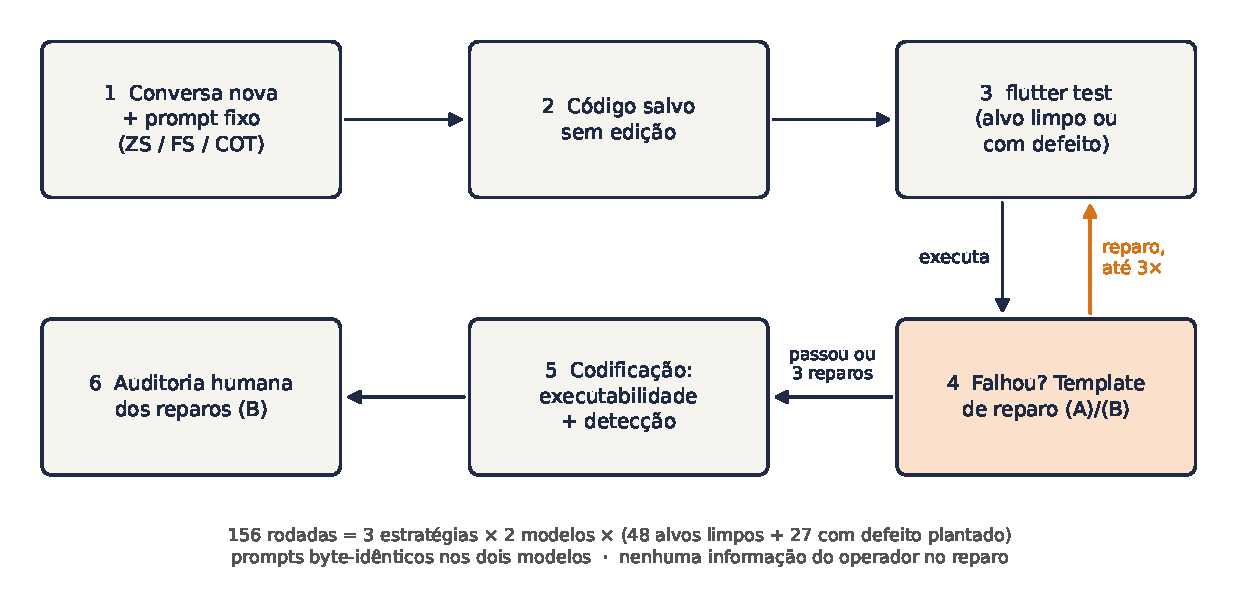
\includegraphics[width=0.95\textwidth]{figuras/fluxograma_metodologia.pdf}
\caption{Protocolo de uma rodada: geração, execução, reparo em duas vias e codificação.}
\label{fig:metodologia}
\end{figure}

A Figura~\ref{fig:metodologia} resume o protocolo de uma rodada, detalhado
na Seção~\ref{subsec:protocolo}. Cada célula alvo~$\times$~estratégia~$\times$~modelo tem uma única rodada.
Trata-se, portanto, de um desenho exploratório sem repetição: os resultados
são descritivos, não se aplicam testes de hipótese e as diferenças entre
modelos e estratégias são lidas por padrões consistentes (por exemplo, 6/6
ou 0/6), não por diferenças percentuais~\cite{baltes2026guidelines}.

\subsection{Declaração de Uso de Modelos de Linguagem}
\label{subsec:declaracao}

Conforme a diretriz 5.1 de Baltes et al.~\cite{baltes2026guidelines},
modelos de linguagem participaram deste trabalho em dois papéis distintos.
(i)~\textbf{Modelos sob estudo}: ChatGPT e Gemini geraram os testes e
autoclassificaram as falhas no ciclo de reparo; são o objeto da comparação.
(ii)~\textbf{Apoio operacional}: o Claude Code (Anthropic) executou os
testes, versionou os artefatos e documentou as rodadas em formato
padronizado, sem editar os testes gerados; na Fase~3, escreveu os três testes
E2E de referência, usados só para provar que os defeitos eram detectáveis
naquele nível e nunca incluídos em \textit{prompt}. O envio dos
\textit{prompts} e a cópia das respostas foram automatizados pela extensão
Claude in Chrome, sem alteração de conteúdo. (iii)~Nenhum modelo de linguagem
participou da codificação de detecção nem da auditoria das
autoclassificações, feitas pelo autor.

\subsection{Objeto de Estudo: o Sintonize}
\label{subsec:sintonize}

O Sintonize é uma aplicação móvel de recomendação musical desenvolvida em
Flutter com \textit{backend} em Firebase (Authentication e Cloud Firestore),
criada por estudantes em uma disciplina de graduação e da qual o autor
participou como desenvolvedor. Oferece cadastro e autenticação de usuários,
recomendação diária de músicas, criação de \textit{playlists}, pesquisa
direta e uma camada social (\textit{Sintonizados}). O cadastro consome a API
pública ViaCEP para preenchimento de endereço. A versão usada é a de
produção do aplicativo, que já havia passado por um processo formal de teste
conduzido pelo autor (matriz de requisitos, plano de teste e planilha de
execução); os defeitos reais que o estudo expõe (Seção~\ref{subsec:res-reais})
são, portanto, defeitos que esse processo não encontrou.

Antes da Fase~2, o aplicativo recebeu uma única alteração estrutural:
as telas \texttt{LoginScreen}, \texttt{CadastroScreen},
\texttt{GenerosCadastroScreen} e \texttt{CriarPlaylistScreen} passaram a
receber as instâncias de \texttt{FirebaseAuth} e \texttt{FirebaseFirestore}
por injeção no construtor, com os valores padrão iguais aos originais. A
mudança não altera o comportamento em execução e torna os testes de
\textit{widget} e integração viáveis com dublês. A tela inicial
(\texttt{TelaInicialScreen}) e as demais permaneceram com acesso estático
ao Firebase, o que se revelou uma limitação de testabilidade recorrente nos
níveis intermediários (Seção~\ref{sec:resultados}). Todo o código sob teste
é o mesmo nos dois modelos e nas duas fases, identificado por \textit{hash}
de \textit{commit} no repositório.

\subsection{Alvos e Defeitos Plantados}
\label{subsec:alvos}

\paragraph{Alvos limpos.} No nível unitário, sete funções de validação de
\texttt{lib/utils/validators.dart} (\texttt{validateNome},
\texttt{validateNumero}, \texttt{validateCEP}, \texttt{validateEmail},
\texttt{validateEmailLogin}, \texttt{validateEmailEdit},
\texttt{validateDate}). A função \texttt{formatName} foi mantida como alvo à
parte porque contém um defeito real pré-existente, identificado no piloto e
não corrigido; suas três rodadas por modelo não entram na contagem de alvos
limpos. Nos níveis de \textit{widget} e integração, três alvos cada,
escolhidos de modo a equilibrar os níveis em três alvos limpos
(Tabela~\ref{tab:desenho}). No nível E2E, os mesmos três fluxos, agora
executados no aplicativo real a partir da tela de boas-vindas.


\paragraph{Defeitos plantados.} Em cada nível foram plantados defeitos dos
dois tipos definidos na Seção~\ref{subsec:oraculo}, CRASH e SILENT, cada um
uma alteração de uma linha. A Tabela~\ref{tab:bugs} lista os nove. As duas
fases usam regimes de oráculo diferentes e complementares. Na \textbf{Fase~2}
o defeito é \emph{visível}: o \textit{prompt} traz o código já alterado,
cuja intenção é evidente no próprio código ou no seu entorno (um comentário
que promete tratar a palavra vazia, uma mensagem que diz ``pelo menos 6''
sob um limite de 7, um nome fixo onde há um campo digitado), e o teste roda
contra esse mesmo código; o que se mede é se o modelo percebe a contradição
e escreve um teste que falha, ou se a fixa como especificação. Os seis
defeitos da Fase~2 ficaram ativos juntos em um único \textit{commit}
(\texttt{295fa34}; código limpo em \texttt{03c9bac}), e a detecção foi
codificada sempre em relação ao defeito-alvo da rodada; a co-atividade é
discutida na Seção~\ref{subsec:ameacas} (I7). Na \textbf{Fase~3} o defeito
é \emph{oculto}: o \textit{prompt} traz o código limpo (\texttt{ccae44a},
idêntico ao limpo da Fase~2) e o teste gerado roda contra um \textit{worktree}
com um único defeito (\texttt{eb14334}, \texttt{20edaaa} e
\texttt{60cbaff}, para L4, C3 e P2); o que se mede é se a suíte gerada é
sensível ao comportamento a ponto de quebrar quando ele muda. A consequência
para a leitura dos resultados é direta: canonizar só é possível no regime
visível, e capturar sem ter visto o defeito só acontece no oculto. A
diferença de regime entre as fases \textbf{não foi planejada}: o desenho
original previa o defeito visível também no E2E; os \textit{prompts} da
Fase~3 foram montados a partir do código limpo e a divergência só foi
percebida na revisão final do texto, quando já não era viável repetir as 36
rodadas. Ela é relatada como desvio (Apêndice~\ref{sec:apendice-desvios}) e
tratada como ameaça de construto (Seção~\ref{subsec:ameacas}, Ct7); o regime
oculto é, por sua vez, o oráculo clássico do teste de mutação, e a leitura
conjunta dos dois regimes acabou por se mostrar informativa. Os critérios de
escolha --- defeito plausível, observável por um teste do nível
correspondente, sem dependência de \textit{timing} --- estão registrados no
repositório. Na Fase~2 os defeitos foram validados por inspeção do código e
pela descrição do sintoma, não por um teste de referência que os detectasse;
na Fase~3, três testes de referência (Seção~\ref{subsec:declaracao})
provaram a detectabilidade de L4, C3 e P2 antes das rodadas. Os defeitos do nível
unitário atingem funções que nenhuma tela chama diretamente (as telas têm
validadores próprios), e por isso são alcançáveis apenas por testes
unitários; os três defeitos do nível E2E foram escolhidos, ao contrário, por
só se manifestarem ao atravessar telas ou após uma resposta real do
\textit{backend}.

\begin{table}[H]
\centering
\caption{Defeitos plantados por nível (uma linha alterada cada). No E2E, L~=~\textit{login}, C~=~cadastro, P~=~\textit{playlist}; o número é o do catálogo de candidatos do repositório.}
\label{tab:bugs}
\small
\begin{tabular}{llP{6.2cm}l}
\toprule
\textbf{ID} & \textbf{Nível} & \textbf{Alteração} & \textbf{Tipo} \\
\midrule
U-CRASH  & Unitário   & \texttt{capitalize}: remove a guarda de palavra vazia ($\to$ \texttt{RangeError}) & CRASH \\
U-SILENT & Unitário   & \texttt{validateSenha}: limite de 6 passa a 7, mensagem inalterada & SILENT \\
W-CRASH  & \textit{Widget} & \texttt{\_filterMusicas}: remove o \textit{null-safety} de \texttt{artist\_name} & CRASH \\
W-SILENT & \textit{Widget} & \texttt{LoginScreen}: mensagens de \textit{user-not-found} e \textit{wrong-password} trocadas & SILENT \\
I-CRASH  & Integração & \texttt{\_salvarGeneros}: \texttt{currentUser!.uid} fora do \texttt{try}, sem guarda & CRASH \\
I-SILENT & Integração & \texttt{\_salvarPlaylist}: nome da \textit{playlist} fixo em vez do digitado & SILENT \\
L4       & E2E        & \textit{login} correto navega para \texttt{CadastroScreen} em vez da \texttt{TelaInicialScreen} & SILENT \\
C3       & E2E        & cadastro grava o e-mail no campo \texttt{nome} do usuário & SILENT \\
P2       & E2E        & lista de músicas com \texttt{itemCount} = tamanho + 1 ($\to$ \texttt{RangeError}) & CRASH \\
\bottomrule
\end{tabular}
\end{table}

\subsection{Estratégias de \textit{Prompt} e Material Fornecido}
\label{subsec:estrategias}

As três estratégias seguem o mesmo esqueleto por nível, e a única variação
entre rodadas de um mesmo alvo é a estratégia. O \textit{prompt} ZS traz a
descrição da tarefa, o código completo do alvo (função, tela ou telas do
fluxo, coladas \textit{verbatim}) e os requisitos de formato e execução. O
\textit{prompt} FS acrescenta, antes da tarefa, um exemplo de teste do mesmo
nível; o COT acrescenta uma sequência de passos de análise (fluxo,
dependências, cenários) a cumprir antes de escrever os testes. Nos níveis de
\textit{widget} e integração, o material inclui as dependências de dublê
disponíveis (\texttt{firebase\_auth\_mocks}, \texttt{fake\_cloud\_firestore},
\texttt{mockito}); no nível E2E, um bloco fixo de ambiente, idêntico nos nove
\textit{prompts}, com o \textit{helper} que aponta o aplicativo para os
emuladores do Firebase, as credenciais e os dados semeados, a navegação a
partir da tela de boas-vindas e o comando de execução.

Os exemplos \textit{few-shot} foram escolhidos conforme a diretriz 5.3 de
Baltes et al.~\cite{baltes2026guidelines}: na Fase~2, um teste de cada nível
vindo dos \textit{templates} do piloto; na Fase~3, um teste
\texttt{integration\_test} de um aplicativo fictício, sobre um fluxo que não
é alvo e sem menção a defeitos.\footnote{O exemplo de integração do piloto
usava uma API inexistente de \texttt{firebase\_auth\_mocks} e foi reescrito
antes da Fase~2; a mudança está registrada na nota de protocolo dos
\textit{prompts}. Um exemplo sempre carrega padrões de prática --- um
caminho de \textit{import}, um laço de espera ---, e essa assimetria é
inerente à estratégia FS; o seu efeito aparece na Seção~\ref{sec:resultados}
e nas ameaças I3 e T4.}

Todos os \textit{prompts} (68 na Fase~2, 9 na Fase~3) são publicados no
repositório com \textit{hash} SHA-256, idênticos byte a byte nos dois
modelos, e cada documento de rodada registra o \textit{hash} do
\textit{prompt} usado. O texto é colado em uma conversa nova, sem
pré-processamento, e o pós-processamento consiste apenas em salvar o bloco de
código sem edição e executá-lo. Os \textit{prompts} têm de 0,6 a 2,3 mil
caracteres no nível unitário, 10 a 28 mil nos níveis intermediários e 34 a
57 mil no E2E (os casos em que a interface não aceitou a entrada estão na
Seção~\ref{subsec:sessao}). O Apêndice~\ref{sec:apendice-prompts} reproduz
o menor e o maior.

\subsection{Protocolo de Rodada e Ciclo de Reparo}
\label{subsec:protocolo}

Cada rodada segue oito passos, documentados em um arquivo padronizado:
(1)~conversa nova no modelo; (2)~colagem do \textit{prompt} sem alteração;
(3)~gravação da resposta integral e do bloco de código, sem edição;
(4)~execução com \texttt{flutter test} (no nível E2E, em um emulador Android
contra os emuladores do Firebase, com os dados semeados e conferidos antes
de cada execução); (5)~se houver falha, envio do \textit{prompt} de reparo,
na mesma conversa; (6)~repetição de (3)--(5) até o sucesso ou até
\textbf{três iterações de reparo}; (7)~arquivamento do teste final e das
saídas de todas as execuções; (8)~codificação da rodada
(Seção~\ref{subsec:metricas}).

O \textit{prompt} de reparo é um \textbf{\textit{template} fixo} que contém
apenas a saída literal do terminal e pede ao modelo que, antes de corrigir,
classifique a causa da falha em \textbf{(A)} o teste presume um
comportamento que não é o especificado, ou \textbf{(B)} o teste capturou um
comportamento potencialmente incorreto da aplicação. Em (A), o modelo corrige
o teste; em (B), é instruído a não enfraquecer a asserção nem reduzir o escopo
do teste, mas a descrever o comportamento observado, o esperado e a suspeita
--- sem alterar o teste. Essa estrutura em duas vias foi a principal revisão
em relação ao piloto, cujo reparo pedia apenas ``corrigir o teste'' e podia
induzir o modelo a acomodar defeitos reais. A classificação declarada pelo
modelo é registrada e, em seguida, \textbf{auditada pelo autor} contra o
código e a saída, separando a correção da \emph{classe} ((A)/(B)) da
correção da \emph{causa} apontada. O \textit{template}, idêntico nas 156
rodadas, é reproduzido na Figura~\ref{fig:template}; o único conteúdo
variável é a saída do terminal.

\begin{figure}[H]
\begin{minipage}{\textwidth}
{\scriptsize
\begin{verbatim}
O teste falhou com o seguinte erro:

```
[COLAR A SAÍDA DE ERRO DO TERMINAL AQUI]
```

Antes de corrigir, classifique a causa provável da falha:
(A) o teste presume um comportamento que não é o especificado, ou
(B) o teste capturou um comportamento potencialmente incorreto da aplicação.
Declare essa classificação explicitamente antes de prosseguir.

Se (A): corrija o teste normalmente.

Se (B): não enfraqueça a asserção nem reduza o escopo do teste para
fazê-lo passar. Descreva o comportamento observado, o comportamento
esperado, e por que você suspeita de um problema na aplicação, em vez de
alterar o teste.
\end{verbatim}
}
\end{minipage}
\caption{\textit{Template} de reparo em duas vias, enviado sem alteração em todas as iterações.}
\label{fig:template}
\end{figure}

Duas regras completam o protocolo. Primeira: o operador \textbf{não
acrescenta informação} ao reparo e não responde a perguntas do modelo; um
reparo (B) sem código resulta na reexecução do arquivo inalterado. Uma rodada
pode, portanto, terminar com um teste falhando de propósito: quando o (B)
procede, esse é o resultado esperado --- o teste capturou o defeito e foi
mantido ---, e a rodada é contada como não verde na executabilidade e como
\emph{Capturou} na detecção. Essa regra
foi violada em 15 rodadas com defeito plantado do ChatGPT na Fase~2, nas
quais o operador forneceu contexto (caminhos, campos reais, nomes de
\textit{widgets}); ao se constatar que a réplica com o Gemini não recebera a
mesma ajuda, as 15 rodadas foram isoladas e \textbf{reexecutadas
integralmente} com o \textit{template} fixo, e são essas reexecuções que
compõem o estudo (Seção~\ref{subsec:ameacas}). Segunda: o código da
aplicação nunca é alterado durante uma rodada, mesmo quando o modelo propõe
mudanças em \texttt{pubspec.yaml} ou nas telas.

\subsection{Modelos, Versões e Condições de Sessão}
\label{subsec:sessao}

Os modelos foram acessados pela interface \textit{web}, que é a condição do
desenvolvedor sem acesso à API e não expõe temperatura, \textit{seed},
\textit{system prompt} nem identificador de \textit{build}. A
Tabela~\ref{tab:versoes} registra, por bloco de rodadas, a versão e a forma
como foi apurada, conforme a diretriz 5.2~\cite{baltes2026guidelines}. A
reprodutibilidade possível é a do protocolo, não a da saída.

\begin{table}[H]
\centering
\caption{Versões e condições de sessão por bloco de rodadas.}
\label{tab:versoes}
\small
\begin{tabular}{P{3.2cm}lP{2.1cm}P{2.9cm}P{3.2cm}}
\toprule
\textbf{Bloco} & \textbf{Modelo} & \textbf{Versão} & \textbf{Fonte} & \textbf{Sessão / período} \\
\midrule
Fase 2, 49 rodadas\textsuperscript{\ddag} & ChatGPT & GPT-5.5/5.6 & autodeclaração & deslogado, set.\ 2026 \\
Fase 2, 15 reexecutadas & ChatGPT & GPT-5.6 Luna & autodeclaração + Help Center & deslogado, 24 set.\ 2026 \\
Fase 2, 64 rodadas\textsuperscript{\ddag} & Gemini & 3.8 Flash & seletor, \textit{print} por sessão & logado (Pro), set.\ 2026 \\
Fase 3, 18 rodadas & ChatGPT & GPT-5.6 Luna & autodeclaração + Help Center & deslogado, 2--6 out.\ 2026 \\
Fase 3, 18 rodadas & Gemini & 3.8 Flash & seletor, \textit{print} por rodada & logado (Pro), 5--6 out.\ 2026 \\
\bottomrule
\multicolumn{5}{p{13.5cm}}{\footnotesize \textsuperscript{\ddag}64 = as 60 rodadas do desenho mais as 4 reexecuções do I-CRASH com \textit{prompt} corrigido (fora das contagens); no ChatGPT, 15 das 64 foram reexecutadas em 24/09 e são as que contam.} \\
\end{tabular}
\end{table}

As condições de sessão diferem entre os modelos por restrição prática: a
sessão deslogada do Gemini não aceitava os \textit{prompts} do estudo e
limitava a conversa a duas respostas, inviabilizando o ciclo de reparo; a
tentativa está documentada no repositório. Segundo a documentação pública da
OpenAI, usuários deslogados recebem o GPT-5.6 Luna, variante de menor custo da
família; o Gemini 3.8 Flash é o modelo padrão do produto. A comparação é,
portanto, entre os \emph{produtos} como o usuário gratuito ou padrão os
encontra, e não entre modelos em paridade de classe --- ameaça tratada na
Seção~\ref{subsec:ameacas}. A versão do ChatGPT mudou de 5.5 para 5.6 durante
a Fase~2 sem aviso, o que é registrado por rodada. O ChatGPT consultou a
\textit{web} por iniciativa própria em algumas gerações e reparos; o fato é
registrado por rodada e não foi controlável na sessão deslogada.

Quando a interface não aceitou a entrada ou devolveu respostas vazias, a
regra foi: até três tentativas idênticas; persistindo a falha, a célula é
registrada como \textbf{sem dado por limitação do serviço} e fica fora da
contagem. Isso ocorreu em duas rodadas E2E do ChatGPT (P2-ZS e C3-COT, com
\textit{prompts} de 50 a 58 mil caracteres) e em uma reexecução do Gemini na
Fase~2. Não se recorreu a sessão logada nem a filtragem da saída, para não
alterar a condição experimental.

\subsection{Infraestrutura de Execução}
\label{subsec:infra}

Os testes dos níveis unitário, de \textit{widget} e de integração foram
executados com \texttt{flutter test} com os dublês indicados nos
\textit{prompts}, em Flutter 3.41.6 (Dart 3.11.4) na quase totalidade das
rodadas; oito rodadas limpas do ChatGPT da Fase~2 (seis unitárias e duas de
integração) e a execução assistida usaram Flutter 3.41.7 (Dart 3.11.5), e uma
rodada do Gemini (WIDGET-COT-03) mudou de versão entre a geração e os
reparos por troca de máquina; cada documento de rodada registra a versão
usada. A reexecução, a Fase~3 e a medição de cobertura usaram 3.41.6. No nível E2E, os testes gerados usam
o pacote \texttt{integration\_test} e rodam o aplicativo real em um emulador
Android (Pixel~6, API~34) contra o Firebase Emulator Suite (Authentication e
Firestore; \texttt{firebase-tools} 15.31.0), com um \textit{helper}
fornecido no \textit{prompt} que redireciona o aplicativo para os emuladores
sem alterar o código de produção. Antes de cada execução, os emuladores são
reiniciados e semeados com um usuário e cinco músicas, e o estado é conferido
por REST. Na Fase~3, cada defeito plantado vive em um \textit{worktree}
próprio, conferido por \texttt{git diff} antes de cada execução. O custo fixo do
ambiente (inicialização do emulador, primeiro \textit{build}) e o custo por
execução foram medidos e são reportados na Seção~\ref{sec:resultados}. A
chamada à API ViaCEP permanece real, por rede externa, e é declarada como
dependência não controlada.

\subsection{Métricas e Codificação}
\label{subsec:metricas}

\paragraph{Executabilidade.} Apurada por rodada e por caso de teste:
\textbf{compilou na geração} (o arquivo gerado compila sem reparo);
\textbf{testes gerados}, contados na geração inicial; \textbf{passando e
falhando} na última execução; \textbf{iterações de reparo}; e \textbf{taxa de
aprovação}, igual a passando~$\div$~(passando~+~falhando) nas rodadas cujo
arquivo final executa --- um arquivo que não compila é contado à parte, com
zero testes passando, e não entra na taxa. Uma rodada é \textbf{verde} quando
o arquivo final executa sem falhas.

\paragraph{Detecção.} Apurada apenas nas rodadas com defeito plantado,
contra o oráculo (o defeito) e, no nível E2E, contra um roteiro manual que
descreve o que um testador veria em cada passo com e sem o defeito. Cada
rodada recebe um único código, pela ordem de precedência da
Tabela~\ref{tab:rubrica}. A rubrica foi escrita antes da codificação e é a
mesma para os dois modelos e para todas as fases; no regime de defeito
oculto (E2E), porém, as categorias que pressupõem que o modelo viu o defeito
--- \textit{Caracterizou com alerta}, \textit{Viu sem asserção} e
\textit{Canonizou} --- não podem ocorrer, e a codificação se reduz a
\textit{Capturou} ou \textit{Não viu}. A categoria
\textit{Canonizou} é a que a taxa de aprovação, sozinha, não distingue de um
teste correto (Seção~\ref{subsec:desenho}).

\begin{table}[H]
\centering
\caption{Rubrica de detecção (ordem de precedência).}
\label{tab:rubrica}
\small
\begin{tabular}{lP{10.3cm}}
\toprule
\textbf{Código} & \textbf{Critério} \\
\midrule
Capturou & O teste falha por causa do defeito e é mantido assim; ou o modelo declara (B) coerente e não acomoda o teste \\
Caracterizou com alerta & A asserção fixa o comportamento com defeito, mas a resposta o nomeia como defeito ou suspeita \\
Viu sem asserção & A resposta nomeia o defeito, mas nenhum teste o exercita \\
Canonizou & A asserção fixa o comportamento com defeito e a resposta não o questiona \\
Não viu & Nenhum teste exercita o cenário do defeito, ou a rodada não chega a ele por erro anterior \\
\bottomrule
\end{tabular}
\end{table}

\paragraph{Autoclassificação.} Para cada iteração de reparo registram-se a
classe declarada pelo modelo ((A)/(B)) e o veredito da auditoria: classe
correta ou falsa e, quando correta, se a causa apontada procede. Reparos (B)
sobre rodadas limpas que a auditoria confirma correspondem a defeitos reais
não plantados, catalogados à parte (Seção~\ref{sec:resultados}).

\paragraph{Análise de erro.} As falhas são categorizadas em: erro de teste
(espera, \textit{finder}, dado inválido), erro de geração (\textit{import},
API inexistente, código truncado), limitação de testabilidade da aplicação,
lacuna de material do \textit{prompt} e limitação do serviço; a frequência
por categoria é reportada, conforme a diretriz 5.5.

\paragraph{Validação e verificação.} Toda codificação de detecção e toda
auditoria de (B) foram feitas por um único avaliador, o autor; a rubrica e o
roteiro manual são publicados para permitir recodificação, e cada código
registrado no documento da rodada aponta para a evidência que o sustenta
(linha da saída de \texttt{flutter test}, asserção do teste final, trecho da
resposta). Não houve segundo avaliador; a limitação é tratada na
Seção~\ref{subsec:ameacas}. Os valores de passando e falhando de cada rodada foram
verificados de forma independente contra a última saída de \texttt{flutter
test} arquivada, nas três fases, sem divergências; na Fase~3, os 86
\textit{prompts} de reparo arquivados --- 85 iterações com resposta nas 34
rodadas com dado, mais o reparo da C3-COT do ChatGPT, enviado três vezes sem
resposta --- foram conferidos byte a byte contra o \textit{template} e as
saídas correspondentes.

\subsection{Material Suplementar}
\label{subsec:suplementar}

O repositório do estudo contém, para cada rodada, o documento padronizado, a
resposta integral do modelo em cada iteração, os \textit{prompts} de reparo
enviados, as saídas de \texttt{flutter test}, o teste final e, quando
aplicável, as capturas de tela; além dos \textit{prompts} com \textit{hash},
das planilhas consolidadas por fase e da pirâmide unificada, dos \textit{branches}
com os defeitos plantados, dos testes de referência da Fase~3 e do roteiro
manual. As conversas da sessão deslogada do ChatGPT não são recuperáveis
após o fechamento da aba; por isso as transcrições foram salvas no momento
da rodada. O repositório está em
\url{https://github.com/MarcosNeto14/sintonize-tcc}, sob licença MIT.

% ============================================================
% RESULTADOS — estudo revisado (Fases 2 e 3), ChatGPT × Gemini
% Fonte dos números: Piramide_Unificada_ChatGPT_x_Gemini.xlsx (aba Rodadas),
% comparacao_chatgpt_x_gemini.md, consolidado_fase3.md, relatorio_bugs.md.
% ============================================================
\section{Resultados}
\label{sec:resultados}

Esta seção apresenta as 156 rodadas do estudo (78 por modelo), organizadas
pela pirâmide: visão geral (\ref{subsec:res-visao}), alvos limpos por nível
(\ref{subsec:res-limpos}), detecção dos defeitos plantados
(\ref{subsec:res-deteccao}), autoclassificação e defeitos reais
(\ref{subsec:res-autoclass}, \ref{subsec:res-reais}), análise de erro
(\ref{subsec:res-erros}), cobertura de código (\ref{subsec:res-cobertura}) e
custo do nível E2E (\ref{subsec:res-custo}).

\paragraph{Convenções.} As rodadas são identificadas por nível, estratégia
e alvo: \texttt{UNIT-COT-06} é a sexta rodada \textit{chain-of-thought} do
nível unitário (alvo \texttt{validateEmailLogin}); \texttt{INT-FS-02}, a
segunda \textit{few-shot} de integração (fluxo de cadastro); as rodadas com
defeito plantado são identificadas pelo defeito e pela estratégia
(\texttt{W-SILENT-FS}, \texttt{C3-COT}). A taxa de aprovação segue a
Seção~\ref{subsec:metricas}: calculada sobre as rodadas cujo arquivo final
executa; um arquivo que não compila (``n.c.'' nas tabelas) é contado à parte,
com zero testes passando. Ficam fora das contagens principais as três rodadas
de \texttt{formatName} por modelo (alvo com defeito real pré-existente,
Seção~\ref{subsec:alvos}) e as quatro rodadas do I-CRASH refeitas com o
\textit{prompt} corrigido (sufixo \texttt{REEXEC};
Seção~\ref{subsec:ameacas}, I2); as 15 rodadas do ChatGPT reexecutadas com o
\textit{template} fixo (Seção~\ref{subsec:protocolo}) substituem as originais
e contam normalmente. No nível E2E, duas células do ChatGPT (P2-ZS e C3-COT)
ficaram sem dado por limitação do serviço (Seção~\ref{subsec:sessao}). T1 a
T4 designam as limitações de testabilidade da aplicação listadas no
Apêndice~\ref{sec:apendice-testabilidade}. ``Tela inicial'' designa a
\texttt{TelaInicialScreen}, destino do \textit{login}; a primeira tela do
aplicativo é a tela de boas-vindas. Todos os valores de passando e falhando
foram verificados contra a última saída arquivada de \texttt{flutter test}.

\subsection{Visão Geral da Pirâmide}
\label{subsec:res-visao}

A Figura~\ref{fig:piramide} mostra a pirâmide implementada; a
Tabela~\ref{tab:piramide-limpos} resume as rodadas com alvo limpo e a
Tabela~\ref{tab:piramide-bugs} as rodadas com defeito plantado, por nível e
modelo. Três padrões atravessam as duas tabelas e organizam o restante da
seção.
\begin{figure}[H]
\centering
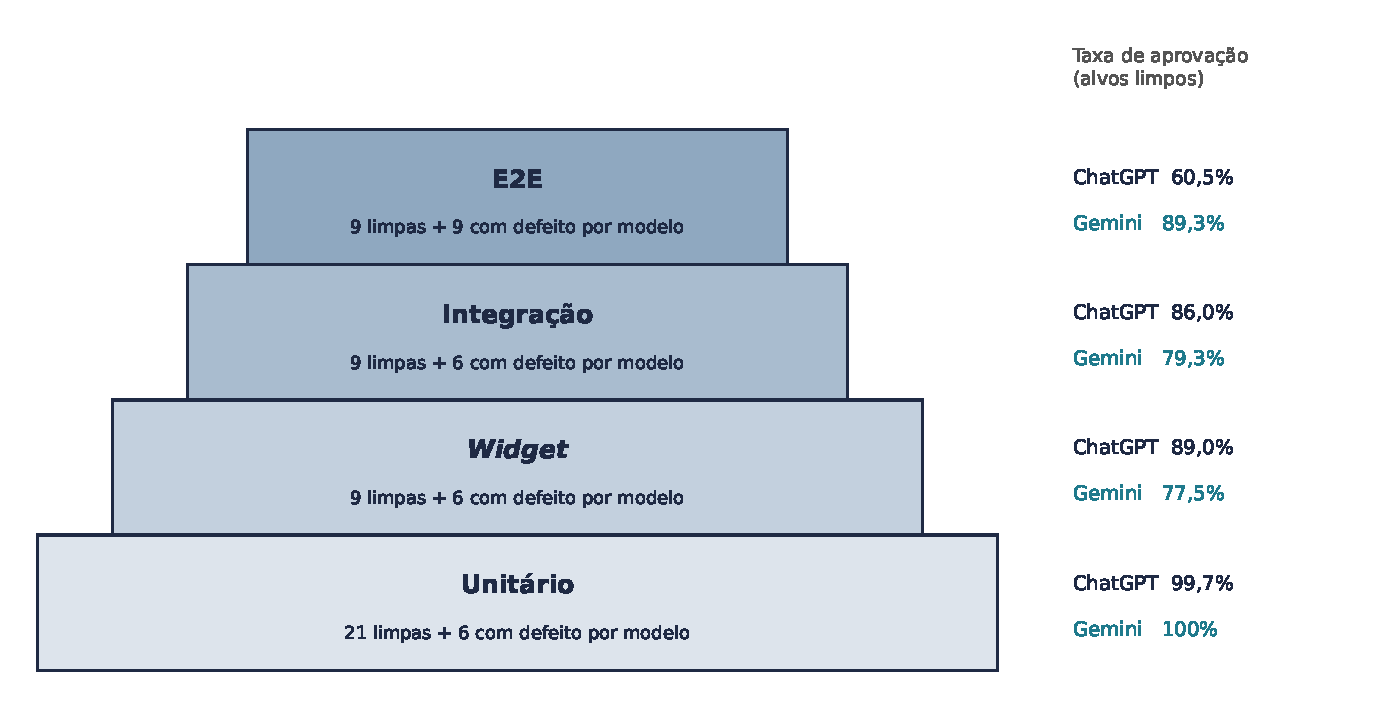
\includegraphics[width=0.8\textwidth]{figuras/piramide_sintonize.pdf}
\caption{A pirâmide implementada: rodadas por nível e por modelo, com a taxa de aprovação nos alvos limpos.}
\label{fig:piramide}
\end{figure}

\begin{table}[H]
\centering
\caption{Alvos limpos por nível e modelo (48 rodadas por modelo).}
\label{tab:piramide-limpos}
\small
\begin{tabular}{llrrrrrr}
\toprule
\textbf{Nível} & \textbf{Modelo} & \textbf{Rod.} & \textbf{Gerados/pass.} & \textbf{Taxa} & \textbf{Verdes} & \textbf{Compilou 1\textsuperscript{a}} & \textbf{Iter.} \\
\midrule
Unitário   & ChatGPT & 21 & 374 / 373 & 99,7\% & 20 & 21 & 6 \\
Unitário   & Gemini  & 21 & 264 / 264 & 100\%  & 21 & 21 & 2 \\
\textit{Widget} & ChatGPT & 9 & 152 / 113 & 89,0\% & 2 & 3 & 24 \\
\textit{Widget} & Gemini  & 9 & 71 / 55   & 77,5\% & 6 & 6 & 17 \\
Integração & ChatGPT & 9 & 50 / 43 & 86,0\% & 4 & 1 & 20 \\
Integração & Gemini  & 9 & 41 / 23 & 79,3\% & 4 & 4 & 20 \\
E2E        & ChatGPT & 9 & 43 / 26 & \textbf{60,5\%} & 3 & 4 & 22 \\
E2E        & Gemini  & 9 & 29 / 25 & \textbf{89,3\%} & 6 & 8 & 17 \\
\midrule
Todos & ChatGPT & 48 & 619 / 555 & 93,4\% & 29 & 29 & 72 \\
Todos & Gemini  & 48 & 405 / 367 & 93,6\% & 37 & 39 & 56 \\
\bottomrule
\multicolumn{8}{p{14cm}}{\footnotesize Gerados/pass.\ = testes gerados na primeira resposta / passando na última execução; Verdes = rodadas cujo arquivo final executa sem falhas; Compilou 1\textsuperscript{a} = rodadas cuja primeira geração compilou; Iter.\ = iterações de reparo somadas.} \\
\end{tabular}
\end{table}

\begin{table}[H]
\centering
\caption{Defeitos plantados por nível e modelo: executabilidade e detecção (rubrica da Tabela~\ref{tab:rubrica}).}
\label{tab:piramide-bugs}
\small
\setlength{\tabcolsep}{3pt}
\begin{tabular}{llrrrrrrrr}
\toprule
\textbf{Nível} & \textbf{Modelo} & \textbf{Rod.} & \textbf{Taxa} & \textbf{Verdes} & \textbf{Capt.} & \textbf{Caract.} & \textbf{Viu s/a.} & \textbf{Canon.} & \textbf{Não viu} \\
\midrule
Unitário   & ChatGPT & 6 & 98,4\% & 5 & 1 & 5 & 0 & 0 & 0 \\
Unitário   & Gemini  & 6 & 100\%  & 6 & 0 & 5 & 1 & 0 & 0 \\
\textit{Widget} & ChatGPT & 6 & 95,3\% & 1 & 0 & 3 & 0 & 0 & 3 \\
\textit{Widget} & Gemini  & 6 & 91,8\% & 3 & 0 & 0 & 0 & 3 & 3 \\
Integração & ChatGPT & 6 & 37,9\% & 2 & 0 & 2 & 1 & 2 & 1 \\
Integração & Gemini  & 6 & 47,6\% & 2 & 0 & 0 & 2 & 2 & 2 \\
E2E        & ChatGPT & 7\textsuperscript{*} & 70,0\% & 0 & \textbf{4} & 0 & 0 & \textbf{0} & 3 \\
E2E        & Gemini  & 9 & 55,2\% & 1 & \textbf{7} & 0 & 0 & \textbf{0} & 2 \\
\midrule
Todos & ChatGPT & 25 & 82,5\% & 8 & 5 & 10 & 1 & 2 & 7 \\
Todos & Gemini  & 27 & 80,8\% & 12 & 7 & 5 & 3 & 5 & 7 \\
\bottomrule
\multicolumn{10}{p{14cm}}{\footnotesize \textsuperscript{*}Mais duas rodadas sem dado por limitação do serviço (Seção~\ref{subsec:sessao}). No E2E o defeito é oculto (\textit{prompt} limpo): Caract., Viu s/a.\ e Canon.\ não se aplicam.}
\end{tabular}
\end{table}

\textbf{Primeiro}, a aprovação agregada dos dois modelos é indistinguível
(93,4\% e 93,6\% nos limpos; 82,5\% e 80,8\% nos defeitos), mas a sua forma
ao longo da pirâmide é diferente: o ChatGPT cai de modo monotônico (99,7
$\to$ 89 $\to$ 86 $\to$ 60\%), enquanto o Gemini cai nos níveis intermediários
e volta a subir no E2E (100 $\to$ 78 $\to$ 79 $\to$ 89\%).
\textbf{Segundo}, a taxa de aprovação esconde a diferença de executabilidade
inicial: a partir do nível de \textit{widget}, o ChatGPT compila na primeira
geração em 8 de 27 rodadas limpas e o Gemini em 18 de 27; o ChatGPT recupera
no reparo, ao custo de 72 iterações contra 56. \textbf{Terceiro}, a detecção
muda de natureza conforme o nível sobe: nos níveis unitário e de
\textit{widget} o modo dominante é \emph{caracterizar} ou \emph{canonizar} o
defeito (o teste passa fixando o comportamento errado); no E2E,
\emph{capturar} passa a ser a norma e nenhuma rodada canonizou --- em parte
por construção, porque no E2E o defeito é oculto e canonizar não é possível
(Seção~\ref{subsec:alvos}). A
Seção~\ref{subsec:res-deteccao} examina esse ponto por defeito.

Em volume, o ChatGPT gerou mais testes que o Gemini em todos os níveis ---
de 1,2 (integração) a 2,1 vezes (\textit{widget}); 1,5 no agregado (619
contra 405 nos limpos; 207 contra 148 nos defeitos) e, por rodada,
gerou mais em 45 das 60 da Fase~2; o volume adicional não se converteu em
aprovação nem em detecção, e sim em iterações.

\subsection{Alvos Limpos por Nível}
\label{subsec:res-limpos}

\paragraph{Unitário.} Os dois modelos compilaram as 21 rodadas na primeira
geração; o Gemini fechou 21 verdes sem reparo em 19 delas e o ChatGPT 20
verdes, com um único teste falhando ao final (\texttt{UNIT-COT-06}, discutido
na Seção~\ref{subsec:res-reais}). O nível não discrimina estratégias nem
modelos; serve de piso.

\paragraph{\textit{Widget}.} É onde a executabilidade inicial se separa: o
ChatGPT compilou 3 de 9 gerações e o Gemini 6 de 9. As causas recorrentes
são as mesmas nos dois modelos --- caminho de \textit{import} inferido para
\texttt{CriarPlaylistScreen} (nenhum dos dois tentou a raiz de \texttt{lib/}),
APIs inexistentes de \texttt{firebase\_auth\_mocks} e a chamada HTTP real da
\texttt{CadastroScreen} à ViaCEP, que fez \texttt{WIDGET-COT-01} nunca
compilar no ChatGPT. O ChatGPT gerou suítes maiores (152 contra 71 testes) e
terminou com apenas 2 rodadas verdes contra 6; a sua taxa mais alta (89\%
contra 77,5\%) vem de suítes grandes com poucas falhas residuais, não de mais
rodadas limpas.

\paragraph{Integração.} O obstáculo é estrutural: a \texttt{TelaInicialScreen},
destino do fluxo de \textit{login}, acessa \texttt{FirebaseAuth.instance}
estaticamente e não pode ser isolada com dublês. Os dois modelos esbarraram
nisso em todas as rodadas do fluxo de \textit{login} e o diagnosticaram como
(B) ou como limitação em 9 rodadas do Gemini e em ao menos 8 do ChatGPT. O
ChatGPT compilou 1 de 9 gerações e o Gemini 4 de 9; ambos fecharam 4 rodadas
verdes. As rodadas FS sem o caminho de \textit{import} formaram um beco nos
dois modelos (4 no ChatGPT e 5 no Gemini, somando \textit{widget} e
integração), com comportamentos opostos: o ChatGPT pediu o caminho e, em duas
rodadas, recusou-se explicitamente a inventar outro; o Gemini tentou três
caminhos e, por fim, colou o próprio \textit{widget} dentro do teste.

\paragraph{E2E.} O nível inverte a tendência do Gemini. Com o aplicativo real
rodando contra os emuladores, desaparecem os três obstáculos dos níveis
intermediários --- dublês, acoplamento estático e caminho de
\textit{import} são substituídos por um \textit{helper} fornecido no
\textit{prompt} --- e o Gemini compila 8 de 9 gerações e fecha 6 rodadas
verdes, duas delas sem nenhum reparo. O ChatGPT, ao contrário, teve o pior
nível: 5 de 9 gerações sem compilar (na maior parte, \texttt{material.dart}
ou o \textit{import} de uma tela ausentes), 3 verdes e 11 reparos
autoclassificados (B), dos quais 9 eram erros do próprio teste. Dois dos
verdes do ChatGPT (\texttt{ZS-03}, \texttt{COT-01}) e um do Gemini
(\texttt{ZS-02}) foram obtidos removendo ou trocando a asserção sobre a
saudação da \texttt{TelaInicialScreen} --- redução de escopo em rodada limpa, permitida sob
(A) pelo \textit{template}, mas que antecipa o modo de falha visto nos
defeitos. Os erros de teste dominantes no E2E, nos dois modelos, foram a
espera insuficiente pela resposta dos emuladores (\texttt{pumpAndSettle}
retorna antes do Auth/Firestore), toques em elementos fora do \textit{viewport}
com o teclado aberto e dados de teste que violam regras presentes no próprio
código colado (nome com dígito, recusado pelo validador da
\texttt{CadastroScreen}).

\paragraph{Por estratégia.} Nenhuma estratégia venceu nos dois modelos. A
Tabela~\ref{tab:estrategias-res} mostra que ZS teve a melhor aprovação nos
dois (95,9\% e 99,4\%); a pior foi FS no ChatGPT (88,0\%), por carregar o
problema do \textit{import} e do \texttt{material.dart}, e COT no Gemini
(88,2\%), com FS logo acima (93,0\%); COT concentrou as consultas espontâneas do ChatGPT à \textit{web} (5 de
6) e as canonizações (5 de 7). A detecção por estratégia é plana: de 4 a 6
rodadas que viram o defeito em cada bloco de 8 ou 9.

\begin{table}[H]
\centering
\caption{Estratégias de \textit{prompt}, todos os níveis (limpos: 16 rodadas por célula; defeitos: 8--9).}
\label{tab:estrategias-res}
\small
\setlength{\tabcolsep}{3.5pt}
\begin{tabular}{llrrrrrr}
\toprule
\textbf{Estr.} & \textbf{Modelo} & \textbf{Taxa (limpos)} & \textbf{Verdes} & \textbf{Compilou 1\textsuperscript{a}} & \textbf{Viu o defeito} & \textbf{Canon.} & \textbf{Não viu} \\
\midrule
ZS  & ChatGPT & 95,9\% & 10 & 11 & 6/8 & 0 & 2 \\
ZS  & Gemini  & 99,4\% & 14 & 13 & 5/9 & 1 & 3 \\
FS  & ChatGPT & 88,0\% &  9 &  9 & 6/9 & 0 & 3 \\
FS  & Gemini  & 93,0\% & 13 & 14 & 6/9 & 1 & 2 \\
COT & ChatGPT & 93,8\% & 10 &  9 & 4/8 & 2 & 2 \\
COT & Gemini  & 88,2\% & 10 & 12 & 4/9 & 3 & 2 \\
\bottomrule
\multicolumn{8}{p{14cm}}{\footnotesize ``Viu o defeito'' = Capturou + Caracterizou com alerta + Viu sem asserção.}
\end{tabular}
\end{table}

\subsection{Detecção dos Defeitos Plantados}
\label{subsec:res-deteccao}

A Tabela~\ref{tab:deteccao-bug} apresenta a codificação de cada uma das 54
rodadas com defeito (27 por modelo), por defeito e estratégia. A leitura por
defeito é mais informativa que a agregada.

\begin{table}[H]
\centering
\caption{Detecção por defeito, estratégia e modelo (passando/falhando no estado final entre parênteses; n.c. = arquivo final não compila).}
\label{tab:deteccao-bug}
\scriptsize
\setlength{\tabcolsep}{3pt}
\begin{tabular}{llP{5.4cm}P{5.4cm}}
\toprule
\textbf{Defeito} & \textbf{Tipo} & \textbf{ChatGPT (ZS $\cdot$ FS $\cdot$ COT)} & \textbf{Gemini (ZS $\cdot$ FS $\cdot$ COT)} \\
\midrule
U-CRASH  & CRASH  & Caracterizou (12/0) $\cdot$ \textbf{Capturou} (5/1) $\cdot$ Caracterizou (12/0) & Caracterizou (11/0) $\cdot$ Viu s/ asserção (6/0) $\cdot$ Caracterizou (10/0) \\
U-SILENT & SILENT & Caracterizou $\times$3 & Caracterizou $\times$3 \\
W-CRASH  & CRASH  & Não viu $\times$3 (14/0, 0/10 n.c., 20/1) & Não viu $\times$3 (5/0, 3/2 n.c., 9/0) \\
W-SILENT & SILENT & Caracterizou $\times$3 (7/1, 0/9 n.c., 0/20 n.c.) & Canonizou $\times$3 (10/1, 9/0, 9/1) \\
I-CRASH  & CRASH  & Viu s/ asserção (1/5) $\cdot$ Não viu (2/1) $\cdot$ Canonizou (2/12) & Não viu (1/4) $\cdot$ Não viu (1/3) $\cdot$ Canonizou (2/4) \\
I-SILENT & SILENT & Caracterizou (2/0) $\cdot$ Caracterizou (0/2 n.c.) $\cdot$ Canonizou (4/0) & Viu s/ asserção (2/0) $\cdot$ Viu s/ asserção (0/2 n.c.) $\cdot$ Canonizou (4/0) \\
L4 & SILENT & \textbf{Capturou $\times$3} (4/1, 1/1, 6/1) & \textbf{Capturou $\times$3} (4/1, 1/1, 5/1) \\
C3 & SILENT & Não viu (3/1) $\cdot$ Não viu (0/1) $\cdot$ sem dado & Não viu (1/2) $\cdot$ \textbf{Capturou} (0/1) $\cdot$ Não viu (5/0) \\
P2 & CRASH  & sem dado $\cdot$ \textbf{Capturou} (0/1) $\cdot$ Não viu (n.c.) & \textbf{Capturou $\times$3} (0/2, 0/1, 0/4) \\
\bottomrule
\end{tabular}
\end{table}

\paragraph{Nível unitário: ver não é proteger.} Os dois defeitos foram
percebidos nas 12 rodadas, mas quase sempre na forma
\emph{Caracterizou com alerta}: o modelo escreve que o comportamento é um
defeito e, na mesma resposta, escreve o teste que o fixa como esperado ---
``o teste deve registrar o comportamento atual'', ``não vou inverter as
asserções''. A única captura por asserção da Fase~2 (ChatGPT, U-CRASH-FS)
veio de um teste que falhou e foi mantido.

\paragraph{W-CRASH: cobertura de dado.} Nenhuma das seis rodadas exercitou o
defeito, porque nenhum teste de busca usou um documento sem o campo
\texttt{artist\_name}. O defeito mede cobertura de dado, não de código, e é
invisível a um gerador que só conhece o esquema pelos exemplos de uso.

\paragraph{W-SILENT: o divisor entre modelos.} Com o mesmo teste --- um caso
por código de erro do Firebase ---, o ChatGPT escreveu em 10 das 12
respostas das três rodadas que as mensagens pareciam invertidas; o Gemini não
escreveu em nenhuma, nem com o \textit{prompt} COT que manda listar cada
mensagem. Nenhum dos dois converteu a suspeita em asserção: os dois fixaram o
par trocado. A diferença está em enxergar uma contradição semântica, não em
agir sobre ela. Na FS, o Gemini foi além: sem o caminho de \textit{import},
declarou dentro do arquivo de teste uma cópia própria da \texttt{LoginScreen},
já com as mensagens trocadas, e as asserções rodam sobre essa cópia --- a
suíte canoniza o defeito sem sequer exercitar a tela real.

\paragraph{I-CRASH e I-SILENT: o pior nível.} O I-CRASH não foi capturado
em nenhuma das seis rodadas originais: nas duas COT os modelos viram o
\texttt{currentUser!.uid} fora do \texttt{try} e escreveram um teste que
fixa a exceção como comportamento esperado; na ZS do ChatGPT o modelo nomeou
a causa certa já na primeira resposta e em um (B), mas o teste que falhava
não alcançava o defeito (caía antes, no formulário divergente do
\textit{prompt}) --- por isso \textit{Viu sem asserção}, e não
\textit{Capturou}. As únicas capturas vieram nas reexecuções com
\textit{prompt} corrigido (ChatGPT ZS e COT), fora das 60. O
I-SILENT foi canonizado em COT nos dois modelos --- o ChatGPT chegou a
acrescentar \texttt{isNot(equals(nome digitado))}, proibindo o comportamento
correto. Nas rodadas ZS e COT desse defeito a suíte passa na primeira
execução e o ciclo de reparo, único ponto do protocolo que proíbe enfraquecer
asserções, nunca é acionado: a canonização nasce na geração.

\paragraph{E2E: captura por construção, exceto no texto.} O L4 foi capturado
nas seis rodadas --- basta afirmar o tipo da tela de destino, e nenhum reparo
(A) retirou essa asserção. O P2 foi capturado nas quatro rodadas que
chegaram à lista de músicas (a quinta com dado, COT do ChatGPT, não compilou): o \texttt{RangeError} entrega arquivo e linha
sem precisar de asserção. O C3, único defeito E2E acomodável por asserção
(um texto na saudação), teve 1 captura em 5 rodadas com dado: só a FS do
Gemini afirmou o campo \texttt{nome} do documento gravado. Três rodadas
caíram antes do sintoma por um dado de teste inválido (nome com dígito,
recusado por regra presente no código colado) e a COT do Gemini chegou à
saudação e afirmou o trecho sem o nome, fechando verde com o defeito ativo.
Em nenhuma rodada E2E houve canonização, e não poderia haver: no regime de
defeito oculto o modelo recebeu o código correto e não tinha o que fixar;
além disso, navegação errada e exceção não são fixáveis por asserção sem
remover o cenário, o que o \textit{template} proíbe sob (B).

\paragraph{Reexecução das 15 rodadas.} A reexecução com \textit{template}
fixo mudou a aprovação, não a detecção: as 15 rodadas somavam 107 testes
passando na execução assistida e 40 na reexecução; quatro que fechavam
verdes terminaram sem compilar. A detecção do ChatGPT quase não se moveu
(W-SILENT continuou visto e fixado nas três; I-SILENT visto nas três;
W-CRASH invisível). A única perda real foi o I-CRASH: sem os campos reais
fornecidos pelo operador, o defeito não foi capturado em nenhuma rodada
original.

\subsection{Autoclassificação (A)/(B)}
\label{subsec:res-autoclass}

O ciclo de reparo produziu 138 iterações na Fase~2 (78 do ChatGPT, 60 do
Gemini) e 85 na Fase~3 (43 e 42). A Tabela~\ref{tab:autoclass} resume as declarações (B) --- as
que afirmam defeito da aplicação --- e o veredito da auditoria.

\begin{table}[H]
\centering
\caption{Reparos autoclassificados (B) e auditoria humana.}
\label{tab:autoclass}
\small
\setlength{\tabcolsep}{4pt}
\begin{tabular}{llP{2cm}rP{4.5cm}P{2.4cm}}
\toprule
\textbf{Fase} & \textbf{Modelo} & \textbf{Contexto} & \textbf{(B)} & \textbf{Classe correta} & \textbf{Causa correta} \\
\midrule
Fase 2 & ChatGPT & limpas & 6\textsuperscript{\dag} & 6 (3 defeitos reais: R2 $\times$2, R5; 3 limitação T1) & 6 \\
Fase 2 & ChatGPT & defeitos plantados & 3 & 1 (I-CRASH-ZS) & 1 \\
Fase 2 & Gemini  & limpas & 7 & 7 (todas limitação T1) & 7 \\
Fase 2 & Gemini  & defeitos plantados & 5 & 1 (I-CRASH-COT) & 0 \\
Fase 3 & ChatGPT & limpas   & 11 & 2 & 2 \\
Fase 3 & ChatGPT & defeitos & 9  & 7 & 2 \\
Fase 3 & Gemini  & limpas   & 7  & 6 & 6 \\
Fase 3 & Gemini  & defeitos & 11 & 11 & 1 (+3 parciais) \\
\bottomrule
\multicolumn{6}{p{14cm}}{\footnotesize \textsuperscript{\dag}A transcrição de WIDGET-COT-02 cita ``(B)'' duas vezes para o mesmo achado; conta-se um.} \\
\end{tabular}
\end{table}

Dois padrões. Nas rodadas com defeito da Fase~3, os dois modelos acertam a
\emph{classe} e erram a \emph{causa} nos defeitos SILENT: nenhum dos 12
reparos (B) sobre o L4 cogitou a rota trocada --- os modelos raciocinam
sobre o \texttt{login.dart} do \textit{prompt}, que está correto, e nunca
consideram que o código em execução difira. No CRASH acertam arquivo e
linha. Nas rodadas limpas, o ChatGPT emite (B) falsos com frequência (9 de
11 na Fase~3) e o Gemini quase não (1 de 7); os (B) corretos em rodada limpa
são defeitos reais não plantados, tratados a seguir, ou limitações de
testabilidade da aplicação (T1, Apêndice~\ref{sec:apendice-testabilidade}). Um
reparo (B) sem código --- 12 ocorrências na Fase~3 --- resulta em reexecução
inalterada e, nos defeitos plantados, é o comportamento desejado.

\subsection{Defeitos Reais Não Plantados}
\label{subsec:res-reais}

Além dos nove defeitos plantados, o estudo expôs cinco defeitos reais do
Sintonize, listados na Tabela~\ref{tab:reais}. Nenhum foi corrigido durante
o estudo, por regra do protocolo; a Seção~\ref{sec:discussao} discute o seu
valor como achado.

\begin{table}[H]
\centering
\caption{Defeitos reais do Sintonize expostos pelo estudo.}
\label{tab:reais}
\scriptsize
\setlength{\tabcolsep}{3pt}
\begin{tabular}{lP{3.5cm}P{4.8cm}P{4.8cm}}
\toprule
\textbf{\#} & \textbf{Local} & \textbf{Defeito} & \textbf{Quem apontou} \\
\midrule
R1 & \texttt{validators.dart} (\texttt{formatName}) e 6 cópias privadas nas telas & \texttt{word[0]} sem guarda para palavra vazia $\to$ \texttt{RangeError} com espaço duplo ou nas pontas & Piloto; Fase 2: ChatGPT caracterizou (ZS, COT), Gemini canonizou (ZS, COT); FS só em prosa nos dois \\
R2 & \texttt{criar\_playlist\allowbreak.dart:169--170} & \texttt{musica['artist\_name'] ?? 'Desconhecido'} é código morto: \texttt{DocumentSnapshot[]} lança \texttt{StateError} antes do \texttt{??}; um documento sem o campo derruba a lista inteira & ChatGPT WIDGET-FS-03, (B) em duas iterações, mantido \\
R3 & \texttt{tela-inicial\allowbreak.dart:161} & \texttt{setState()} após \texttt{dispose()}, sem \texttt{mounted} & Gemini FS-01, FS-02, COT-01 (diagnóstico exato); ChatGPT FS-01, ZS-01 \\
R4 & \texttt{criar\_playlist\allowbreak.dart:38--48} & \texttt{setState} sem \texttt{mounted} e \texttt{catch} que só faz \texttt{print}: um defeito de tratamento de erro escondendo outro & ChatGPT COT-03 (pelo efeito), P2-COT \\
R5 & \texttt{validators.dart:105} e \texttt{login.dart:124} & regex de e-mail sem \texttt{\$}: aceita \texttt{'a@b.com x'} e \texttt{' a@b.com'} & ChatGPT UNIT-COT-06: capturado por um teste e canonizado por outro da mesma suíte (ver texto) \\
\bottomrule
\end{tabular}
\end{table}

R5 merece registro literal: o modelo escreveu um teste chamado ``valida
e-mail com espaços antes/depois (sem trim)'', afirmou \texttt{isNull} para
\texttt{' test@example.com '} e comentou ``regex ainda considera válido
porque não há trim''. Na mesma suíte, outro teste --- e-mail com espaço no
domínio --- falhou, foi classificado (B) com a causa exata (classe
\texttt{[\^{}@]+} sem excluir espaço, regex sem \texttt{\$}) e mantido. O
mesmo defeito foi capturado por um teste e canonizado pelo vizinho: é a forma
mais pura do fenômeno que o estudo mede --- o defeito foi visto, nomeado e,
em parte, transformado em especificação.

\subsection{Análise de Erro}
\label{subsec:res-erros}

Seguindo a diretriz 5.5 de Baltes et al.~\cite{baltes2026guidelines}, as
falhas foram categorizadas. A Tabela~\ref{tab:erros} dá a frequência por
categoria nas duas fases: na Fase~2, rodadas afetadas em 120 (60 por
modelo, sem REEXEC) e, separadamente, a categoria da primeira falha; na Fase~3,
gerações sem compilar e categoria dominante.

\begin{table}[H]
\centering
\caption{Categorias de falha e frequência (rodadas afetadas).}
\label{tab:erros}
\small
\setlength{\tabcolsep}{4pt}
\begin{tabular}{P{2.3cm}P{3.7cm}P{4.3cm}P{2.7cm}}
\toprule
\textbf{Categoria} & \textbf{Exemplos} & \textbf{Fase 2 (ChatGPT / Gemini)} & \textbf{Fase 3 (ChatGPT / Gemini)} \\
\midrule
Erro de geração & \textit{import} de tela, \texttt{material.dart}, API inexistente, código truncado & 27 / 15 afetadas; 1\textsuperscript{a} falha em 25 / 14 & 9 / 2 gerações sem compilar \\
Erro de teste & espera insuficiente, \textit{finder} fora do \textit{viewport}, dado inválido, asserção um quadro cedo & 25 / 21 afetadas; 1\textsuperscript{a} falha em 8 / 10 & dominante nos dois \\
Limitação de testabilidade & \texttt{FirebaseAuth\allowbreak.instance} estático, ViaCEP real, item do \textit{dropdown} fora do \textit{viewport} & 16 / 13 afetadas; 1\textsuperscript{a} falha em 0 / 2 & ViaCEP (SnackBar) em cadastro \\
Lacuna de material & caminho de \textit{import} (FS); material divergente do I-CRASH & 6 / 8 afetadas (nunca causa imediata: aparece como \textit{import} ou \textit{finder}) & --- \\
Limitação do serviço & recusas, respostas vazias, limite de entrada & 1 / 22 afetadas (21 recusas em 17 rodadas) & 2 células sem dado / 0 \\
Não determinismo do E2E & mesma suíte, resultados diferentes & --- & COT-02 (6/11 e 4/11); FS-02 (0/1 $\to$ 1/1) \\
\bottomrule
\end{tabular}
\end{table}

Dos 14 ``Não viu'' da pirâmide, 9 são cenário nunca coberto (W-CRASH nos
dois modelos, I-CRASH sem o teste escrito), 3 são rodadas derrubadas antes do
sintoma por um dado de teste inválido (o nome com dígito), 1 não compilou
(P2-COT do ChatGPT) e 1 chegou ao sintoma sem afirmá-lo. Ou seja, o principal obstáculo à detecção não foi
reconhecer o defeito, e sim chegar até ele.

\subsection{Cobertura de Código}
\label{subsec:res-cobertura}

Como métrica complementar e estabelecida~\cite{baltes2026guidelines}, a
cobertura de linhas dos testes finais das rodadas limpas foi medida em
2026-10-07 com \texttt{flutter test --coverage}, um arquivo por vez, sobre o
\texttt{lib/} limpo (Fase~2: 75 de 78 arquivos medidos, 3 não compilam ou não
carregam; Fase~3: 18 de 18, no emulador com os emuladores do Firebase). A
cobertura é a da execução da medição e foi coletada independentemente de o
teste passar; no E2E, três arquivos do ChatGPT (playlist) falharam na
medição apesar de dois deles terem fechado verdes na rodada --- instabilidade
entre dias, registrada e não corrigida. A Tabela~\ref{tab:cobertura}
apresenta duas leituras: a \textbf{união da célula} (linhas do aplicativo
inteiro, 1\,657 instrumentadas, cobertas por pelo menos uma das três rodadas
da célula) e a \textbf{cobertura média dos arquivos do alvo} (as telas do
fluxo ou \texttt{validators.dart}), que mede quanto do que foi pedido o teste
exercita.

\begin{table}[H]
\centering
\caption{Cobertura de linhas das rodadas limpas: união da célula sobre o aplicativo e média sobre os arquivos do alvo.}
\label{tab:cobertura}
\small
\begin{tabular}{llrrrr}
\toprule
& & \multicolumn{2}{c}{\textbf{União, app (\%)}} & \multicolumn{2}{c}{\textbf{Média, arquivos do alvo (\%)}} \\
\textbf{Nível} & \textbf{Estr.} & ChatGPT & Gemini & ChatGPT & Gemini \\
\midrule
Unitário   & ZS/FS/COT & 69,6\textsuperscript{a} & 69,6\textsuperscript{a} & --- & --- \\
\textit{Widget} & ZS  & 29,0 & 26,3 & 77,9 & 70,9 \\
\textit{Widget} & FS  & 25,9 & 30,2 & 69,7 & 81,0 \\
\textit{Widget} & COT & 21,2\textsuperscript{b} & 28,7 & 75,2\textsuperscript{b} & 77,1 \\
Integração & ZS  & 26,6 & 31,1\textsuperscript{c} & 74,6 & 86,0\textsuperscript{b} \\
Integração & FS  & 22,4 & 6,2  & 65,9 & 43,0\textsuperscript{b} \\
Integração & COT & 28,1 & 25,6\textsuperscript{b} & 78,8 & 94,3\textsuperscript{b} \\
E2E        & ZS  & 21,1\textsuperscript{d} & 40,4 & 39,9\textsuperscript{d} & 76,4 \\
E2E        & FS  & 24,4\textsuperscript{d} & 40,3 & 47,0\textsuperscript{d} & 77,5 \\
E2E        & COT & 38,9\textsuperscript{d} & 41,0 & 63,0\textsuperscript{d} & 83,9 \\
\bottomrule
\multicolumn{6}{p{14.5cm}}{\footnotesize \textsuperscript{a}Denominador = \texttt{validators.dart} (46 linhas); as 14 linhas não cobertas são de funções fora dos alvos limpos.} \\
\multicolumn{6}{p{14.5cm}}{\footnotesize \textsuperscript{b}Menos de 3 rodadas medidas (arquivo não compila, não carrega ou não carregou o alvo). \textsuperscript{c}Denominador 296: as rodadas não importam \texttt{main.dart}.} \\
\multicolumn{6}{p{14.5cm}}{\footnotesize \textsuperscript{d}Playlist do ChatGPT com 0 testes passando na medição (ZS instável: 1/1 e 384 linhas na repetição).} \\
\end{tabular}
\end{table}

Três leituras. Primeira, \textbf{no nível unitário a cobertura não
discrimina nada}: as três estratégias e os dois modelos cobrem exatamente as
mesmas 32 linhas de \texttt{validators.dart} --- as funções-alvo são pequenas e
qualquer suíte que compile as percorre inteiras. Segunda, \textbf{o volume
não vira cobertura}: o ChatGPT gerou 1,5 vez mais testes no agregado e
cobriu menos linhas do aplicativo que o Gemini em 6 das 9 células de
\textit{widget}, integração e E2E (nas outras 3, mais por 2 a 3 pontos em
\textit{widget} ZS e integração COT, e em integração FS porque o arquivo do
Gemini quase não executou); no E2E só se aproxima do Gemini em COT (38,9\%
contra 41,0\%), onde gerou suas suítes maiores. Terceira, \textbf{a
cobertura dos arquivos do alvo é alta nos dois modelos onde o teste
executa} (66--94\% em \textit{widget} e integração, com uma exceção: a FS
de integração do Gemini, 43\%, uma rodada medida), o que confirma que o
obstáculo é chegar a executar, não escolher o que exercitar; no E2E, a
diferença entre modelos (40--63\% contra 76--84\%) reflete sobretudo as
suítes do ChatGPT que falharam cedo na medição. A cobertura, como a taxa de
aprovação, nada diz sobre detecção: as suítes que canonizaram o I-SILENT
cobrem \texttt{\_salvarPlaylist} por inteiro.

\subsection{Custo do Nível E2E}
\label{subsec:res-custo}

Uma execução E2E levou de 20 a 90~s de teste mais 11 a 75~s de
\textit{build} incremental; uma rodada completa (até quatro execuções e três
reparos) cerca de 45~min com envio automatizado. O custo fixo do ambiente
foi de 132~s para iniciar o emulador Android e 362~s para o primeiro
\textit{build}; a configuração inicial (SDK, emulador, Firebase CLI, \textit{flag}
de hipervisor) exigiu privilégios de administrador e cerca de 7~h de trabalho
(28/09/2026). Os
\textit{prompts} E2E têm de 34 a 57 mil caracteres, e os reparos chegaram a
141 mil (aceitos pelo Gemini); no ChatGPT deslogado, entradas acima de 50 mil
caracteres falharam de forma intermitente, o que produziu as duas células
sem dado. O esforço humano por rodada não foi cronometrado; o intervalo
entre \textit{commits} de documentação de rodadas consecutivas, estimado
sobre 172 \textit{commits}, tem mediana de 9 a 15~min por rodada na Fase~2 e
no E2E do ChatGPT e de 30~min no E2E do Gemini (com envio automatizado em
cerca de 80\% das rodadas). O número mede o ritmo de executar e documentar,
não o tempo de auditoria e codificação, que ficou sem medida.

\subsection{Síntese}
\label{subsec:res-sintese}

(1)~A taxa de aprovação não separa modelos nem estratégias; a
executabilidade na primeira geração e o esforço de reparo separam os
modelos a partir do nível de \textit{widget}, a favor do Gemini.
(2)~A detecção depende do regime do oráculo, do tipo de defeito e de uma
asserção específica, não da estratégia: no E2E (defeito oculto), exceção e
navegação errada são capturadas por todas as rodadas que as alcançam; nos
níveis inferiores (defeito visível), CRASH e SILENT são igualmente
caracterizados, canonizados ou ignorados.
(3)~O ChatGPT vê mais e diz mais (W-SILENT, 10 de 12 respostas), mas isso
não vira asserção; o Gemini canoniza em silêncio com mais frequência.
(4)~Nos defeitos plantados, nenhum reparo (B) enfraqueceu um teste; as
canonizações nascem na geração, antes do reparo, e as reduções de escopo
ocorrem em rodadas limpas sob (A).
(5)~O nível E2E, mais caro e sob o regime de defeito oculto, foi o único em
que a captura é a norma --- e o
único em que o Gemini supera o seu próprio desempenho nos níveis
intermediários, porque o aplicativo real elimina os obstáculos de
testabilidade que os dublês criavam.
(6)~O estudo expôs cinco defeitos reais, um deles transformado em
especificação por um teste gerado.

% ============================================================
% DISCUSSÃO E AMEAÇAS À VALIDADE — estudo revisado (Fases 2 e 3)
% Fonte: piramide_unificada.md §4, relatorio_bugs.md, limitacoes_validade.md,
% medeiros2026_resumo_e_uso.md, baltes2026_aplicacao_tcc.md.
% ============================================================
\section{Discussão}
\label{sec:discussao}

\subsection{Resposta à Questão de Pesquisa}
\label{subsec:disc-qp}

A questão de pesquisa tem duas partes: em que medida modelos de linguagem,
guiados por estratégias de \textit{prompt}, implementam uma pirâmide de testes
que de fato protege uma aplicação móvel real; e quais são os desafios
encontrados em cada nível. A primeira parte tem três respostas; a segunda é
respondida nível a nível na Tabela~\ref{tab:desafios}.

\paragraph{Implementar, sim; proteger, nem sempre.} Os dois modelos
produziram, em todos os níveis, suítes que compilam e passam --- 93\% de
aprovação agregada nos alvos limpos, com 29 e 37 rodadas verdes em 48. Mas a
mesma pirâmide, medida pela capacidade de detectar defeitos conhecidos,
mostra outra coisa: das 27 exposições a defeito por modelo (nove defeitos
$\times$ três estratégias), o ChatGPT capturou 5 e o Gemini 7; os demais foram caracterizados com alerta (10 e 5), canonizados
(2 e 5), vistos apenas em prosa (1 e 3) ou não vistos (7 e 7). Um leitor que
tivesse apenas a taxa de aprovação concluiria que a pirâmide está pronta;
um leitor que tivesse apenas a detecção concluiria que ela protege contra
pouco mais de um quinto das exposições a defeito --- cerca de três em cada
cinco, se contar os casos em que o modelo apenas avisou em prosa ---, e contra quase nenhum dos
silenciosos nos níveis intermediários. As duas leituras são verdadeiras e precisam coexistir no
texto --- é a razão de o estudo medir as duas dimensões em separado.

\paragraph{A estratégia de \textit{prompt} não é o fator decisivo.} ZS, FS e
COT não produziram ordenação consistente entre os dois modelos em nenhuma
métrica. FS foi a pior em aprovação no ChatGPT e a segunda pior no Gemini,
mas por uma razão que não é da estratégia: o exemplo deslocava o modelo para um caminho de
\textit{import} que não existia (Fase~2) ou para um esqueleto sem
\texttt{material.dart} (Fase~3). COT concentrou as canonizações e as
consultas espontâneas à \textit{web}; a sua instrução de ``listar cada
mensagem'' não fez o Gemini perceber as mensagens trocadas do W-SILENT. A
detecção por estratégia é plana. O que variou de verdade foi o material
colado no \textit{prompt} e o tipo de defeito.

\paragraph{O regime do oráculo e o tipo de defeito decidem a detecção.}
No regime de defeito oculto (E2E), exceção (P2) e navegação errada (L4)
foram capturadas em todas as rodadas que as alcançaram, em qualquer
estratégia e modelo, porque derrubam o teste sem depender de asserção; o
defeito de texto (C3) só foi capturado onde uma asserção afirmou o campo
certo. No regime de defeito visível (níveis inferiores), o tipo deixa de
proteger: os CRASH foram tão fixados quanto os SILENT --- U-CRASH
caracterizado em 5 de 6, I-CRASH canonizado nas duas COT, W-CRASH nunca
exercitado ---, porque o modelo, ao ler o código errado, escreve o teste que
o espera. Isso explica a Tabela~\ref{tab:piramide-bugs} melhor do que
qualquer diferença entre modelos: no E2E a captura virou a norma e a
canonização desapareceu por construção, não por mérito do nível.

\paragraph{Os desafios por nível.} A Tabela~\ref{tab:desafios} responde à
segunda parte da questão. O desafio muda de natureza ao subir a pirâmide: no
nível unitário é de \emph{julgamento} (o modelo vê o defeito e não o
protege); nos níveis intermediários é de \emph{infraestrutura de teste}
(dublês, acoplamento estático, material do \textit{prompt}); no E2E é de
\emph{execução} (espera, dispositivo, custo), e a detecção, que era o
problema embaixo, passa a ser dada pela natureza dos defeitos.

\begin{table}[H]
\centering
\caption{Desafio dominante em cada nível, com a causa e a evidência.}
\label{tab:desafios}
\small
\setlength{\tabcolsep}{4pt}
\begin{tabular}{P{1.7cm}P{4.1cm}P{4.5cm}P{3.2cm}}
\toprule
\textbf{Nível} & \textbf{Desafio dominante} & \textbf{Causa} & \textbf{Evidência} \\
\midrule
Unitário & Ver sem proteger: os dois defeitos foram percebidos nas 12 rodadas, mas capturados em uma; nas demais a asserção fixa o comportamento do código fornecido e a resposta apenas avisa & O modelo trata o código colado como especificação (``o teste deve registrar o comportamento atual'') & Tabela~\ref{tab:piramide-bugs}; Seção~\ref{subsec:res-deteccao} \\
\addlinespace
\textit{Widget} & Compilar na primeira geração (ChatGPT 3 de 9, Gemini 6 de 9) e exercitar o dado certo: W-CRASH invisível nas seis rodadas & Caminho de \textit{import} inferido, APIs de dublê inexistentes, chamada real à ViaCEP (T3); nenhum teste de busca usa documento sem o campo & Tabela~\ref{tab:piramide-limpos}; Tabela~\ref{tab:erros} \\
\addlinespace
Integração & Testabilidade: pior aprovação com defeito (37,9\% e 47,6\%) e 10 dos 13 (B) corretos em rodadas limpas são a limitação T1; I-SILENT canonizado já na geração & \texttt{FirebaseAuth\allowbreak.instance} estático na \texttt{TelaInicialScreen}, não isolável com dublê; material divergente do I-CRASH & Tabela~\ref{tab:autoclass}; Tabela~\ref{tab:piramide-bugs}; Apêndice~\ref{sec:apendice-testabilidade} \\
\addlinespace
E2E & Execução e custo: 5 de 9 gerações do ChatGPT sem compilar, erros de espera e de \textit{viewport}, resultados não determinísticos, duas células sem dado; a detecção, ao contrário, é a norma (L4 6/6, P2 4/5), exceto no defeito de texto (C3 1/5) & \texttt{material.dart} ausente; \texttt{pumpAndSettle} antes da resposta dos emuladores; dado de teste que viola regra do código colado; \textit{prompts} de 34 a 57 mil caracteres no serviço deslogado & Seções~\ref{subsec:res-limpos} e \ref{subsec:res-custo}; Tabelas~\ref{tab:erros} e \ref{tab:deteccao-bug} \\
\bottomrule
\end{tabular}
\end{table}

\subsection{Canonização: o Modo de Falha}
\label{subsec:disc-canon}

Chama-se aqui canonização o teste que fixa um defeito como comportamento
esperado. O estudo observou sete casos nos defeitos plantados (2 do ChatGPT,
5 do Gemini), mais o R5 em alvo limpo, e três achados sobre ela importam para quem usa modelos de
linguagem em testes.

Primeiro, \textbf{ela nasce na geração, não no reparo} --- e nasce porque,
no regime de defeito visível, o modelo lê o código errado e o toma como
especificação. O \textit{template}
de reparo em duas vias --- a revisão feita após o piloto --- cumpriu o que
prometia: em 52 rodadas com defeito e dado, nenhum
reparo (B) enfraqueceu uma asserção, e reparos (B) sem código resultaram em
reexecução inalterada. Mas o \textit{template} só é acionado quando um teste
falha; nas rodadas ZS e COT do I-SILENT a suíte passou na primeira
execução, já canonizada, e o reparo nunca entrou. Nas sete canonizações, a
asserção que fixa o defeito já estava na primeira resposta do modelo
(conferido contra as transcrições; em três rodadas do Gemini, contra o
trecho registrado no documento da rodada, por não haver o arquivo da
iteração~0); em uma delas (I-CRASH COT do Gemini) a asserção foi
enfraquecida em um reparo intermediário e restaurada no seguinte. Um protocolo que quisesse
atacar a canonização teria de agir no \textit{prompt} de geração --- por
exemplo, pedindo que o modelo liste os comportamentos que considera
suspeitos antes de escrever as asserções.

Segundo, \textbf{ver e proteger não são a mesma coisa}. O ChatGPT escreveu
que as mensagens do W-SILENT pareciam invertidas em 10 das 12 respostas e,
nas mesmas respostas, escreveu o teste que as fixa; justificou-se: ``o
teste deve registrar o comportamento atual''. O Gemini não viu a troca em
nenhuma. A diferença entre os modelos está na percepção de uma contradição
semântica, não na ação sobre ela --- e é por isso que a categoria
\emph{Caracterizou com alerta} existe na rubrica: sem ela, o ChatGPT e o
Gemini pareceriam iguais no W-SILENT, quando um deles entregou ao
desenvolvedor a informação de que algo está errado e o outro não.

Terceiro, \textbf{a canonização de um defeito real é indistinguível de uma
especificação}. O R5 é o caso-limite: o modelo nomeou o defeito no título do
teste, explicou-o num comentário e afirmou o comportamento errado como
esperado. Esse teste passa, está bem escrito e documenta um defeito como
regra do sistema. Nenhuma métrica de executabilidade o distingue de um teste
correto; só um revisor humano que leia o teste contra a intenção do código.

\subsection{Material do \textit{Prompt} e o que o Modelo Faz sem Ele}
\label{subsec:disc-material}

Nas duas fases, uma fonte recorrente de rodadas perdidas foi informação que o
modelo não tinha ou não usou. Na Fase~2, o caminho de \textit{import} do
alvo (FS) e o material divergente do I-CRASH; na Fase~3, o \textit{import}
de \texttt{material.dart} e das telas, e um dado de teste que violava uma
regra presente no próprio código colado. Diante da lacuna, os dois modelos
reagiram de formas opostas e consistentes (Seção~\ref{subsec:res-limpos}):
o ChatGPT pediu ou recusou; o Gemini inventou. O resultado foi o mesmo ---
arquivo que não compila ---, mas o comportamento tem consequências
diferentes para quem opera: a recusa é
visível e corrigível com uma linha; a invenção produz um artefato que parece
um teste e não testa o alvo.

Medeiros~\cite{medeiros2026acessibilidade}, no nível E2E de portais
\textit{web} com o Gemini 3 Flash, chegou ao mesmo ponto por outro caminho:
os \textit{scripts} melhoraram quando o \textit{prompt} passou a fornecer os
seletores reais da interface e a proibir a sua invenção. Os dois estudos
convergem numa regra prática: o que o modelo não recebe no \textit{prompt},
ele inventa ou trava, e o esforço humano migra da escrita do teste para a
validação do teste.

Há um corolário incômodo para o desenho do estudo. Fornecer o caminho de
\textit{import} e os campos reais teria aumentado a aprovação --- a execução
assistida da Fase~2 mostra o tamanho do efeito
(Seção~\ref{subsec:res-deteccao}). Mas teria medido o par operador~+~modelo,
e não o modelo; reexecutar as 15 rodadas, com perda de aprovação e
preservação da detecção, foi a escolha de medir o construto certo ao custo de
números piores.

\subsection{A Forma da Pirâmide por Modelo}
\label{subsec:disc-piramide}

O resultado não antecipado é a curva do Gemini: pior que o ChatGPT
nos níveis de \textit{widget} e integração em aprovação, e melhor no E2E
(89\% contra 60\%, 6 verdes contra 3, 8 contra 4 compilações na primeira
geração). A explicação está no que cada nível exige além de escrever
testes. Os níveis intermediários exigem dominar dublês de Firebase, APIs de
\textit{mock} com nomes parecidos e um acoplamento estático que não se
isola; o E2E, com o aplicativo real e um \textit{helper} fornecido, exige
apenas navegar e esperar. O Gemini erra mais no primeiro conjunto de
habilidades e menos no segundo; o ChatGPT, ao contrário, gera suítes maiores
e mais ambiciosas em todos os níveis e paga por isso no E2E, onde cada
teste a mais é mais uma oportunidade de \textit{import} ausente, toque fora
do \textit{viewport} ou espera insuficiente. A pirâmide, como metáfora de
proporção, pressupõe que o custo cresce com o nível; para um gerador
automático, o que cresce com o nível é a dependência de infraestrutura, e
ela pode favorecer ou punir um modelo independentemente da sua capacidade
de escrever testes.

Esse ponto tem uma consequência metodológica: comparar modelos por um só
nível da pirâmide --- como faz a maior parte dos trabalhos relacionados ---
produziria uma ordenação diferente conforme o nível escolhido. No nível de
\textit{widget} o ChatGPT ``vence'' em taxa; no E2E o Gemini vence em tudo;
no unitário, empatam. Só a pirâmide inteira mostra que nenhum dos dois
domina.

\subsection{Defeitos Reais e o Valor do Experimento}
\label{subsec:disc-reais}

Os cinco defeitos reais não eram o objetivo e são, talvez, o resultado de
maior utilidade prática: sobreviveram ao processo formal de teste que o
próprio autor conduziu sobre a versão de produção (Seção~\ref{subsec:sintonize}). Três foram diagnosticados corretamente por pelo
menos um modelo (R1, R2, R3) --- no caso do R3, com arquivo, linha e a
palavra \texttt{mounted} ---, um só pelo efeito (R4) e um foi, na mesma rodada, capturado por um teste e
canonizado por outro (R5). O R1 revelou-se maior do que o piloto indicava: além de
\texttt{formatName}, seis cópias privadas do mesmo laço, alimentadas por
dados do Firestore, carregam o mesmo \texttt{RangeError}. O R2 e o R4 têm em
comum um padrão de tratamento de erro que esconde a causa --- um \texttt{??}
que nunca executa, um \texttt{catch} que só imprime ---, e foram expostos
porque os testes gerados exercitaram caminhos que o desenvolvimento manual
não exercitou. Para a equipe do Sintonize, o relatório da
Tabela~\ref{tab:reais} é um produto direto do estudo; para o estudo, os
cinco casos são a contraprova de que o oráculo plantado não é artificial: os
modelos encontram defeitos que ninguém plantou, e os tratam da mesma forma
que tratam os plantados.

\subsection{Comparação com os Trabalhos Relacionados}
\label{subsec:disc-relacionados}

O mecanismo de reparo por realimentação de erro é o do
TestPilot~\cite{schafer2024testpilot}, e os resultados convergem em um ponto
que aquele trabalho registra de passagem: parte dos testes que passam o
fazem por asserções fracas. Aqui esse fenômeno foi medido com um oráculo e
recebeu nome e taxonomia --- sete canonizações em 52 rodadas com defeito e
dado, mais
um defeito real transformado em especificação --- e mostrou-se concentrado na
geração, fora do alcance do reparo. Plein et al.~\cite{plein2023bugreports}
usam múltiplas gerações como recuperação; o ciclo de reparo deste trabalho
tem o mesmo papel, com a diferença de que cada iteração é auditada e a
classe declarada pelo modelo ((A)/(B)) é ela própria um dado. Os trabalhos de
teste de GUI móvel com LLM~\cite{liu2024gptdroid,yoon2024droidagent,liu2023qtypist}
medem exploração --- atividades visitadas, \textit{bugs} encontrados --- e
produzem \textit{traces}, não suítes; o nível E2E deste trabalho pergunta o
contrário: se uma suíte repetível, gerada de uma vez, protege contra um
defeito conhecido. A comparação mais direta é com
Medeiros~\cite{medeiros2026acessibilidade}, feita na
Seção~\ref{subsec:disc-material}. Nenhum dos trabalhos relacionados cobre os quatro níveis no
mesmo sistema, usa defeitos plantados como oráculo ou compara dois modelos
sob \textit{prompts} idênticos byte a byte; são as três lacunas da
Seção~\ref{sec:relacionados}, e são o que a Tabela~\ref{tab:piramide-bugs}
preenche.

\subsection{Ameaças à Validade}
\label{subsec:ameacas}

As ameaças são organizadas segundo os quatro tipos da diretriz 5.8 de
Baltes et al.~\cite{baltes2026guidelines}, com a mitigação adotada em cada
caso. O repositório do estudo contém a lista completa, incluindo os desvios
operacionais menores.

\paragraph{Validade externa.} (E1)~\emph{Condições de sessão distintas}: o
ChatGPT foi usado deslogado (GPT-5.6 Luna, a variante de menor custo da
família) e o Gemini logado em conta Pro (3.8 Flash, o modelo padrão do
produto). A comparação é entre os produtos como o usuário gratuito ou padrão
os encontra, não entre modelos em paridade de classe; a condição foi mantida
constante dentro de cada modelo e em cada fase, e a tentativa deslogada do
Gemini está documentada. (E2)~\emph{Instabilidade temporal}: o ChatGPT mudou
de 5.5 para 5.6 durante a Fase~2 sem aviso; nenhuma interface expõe
parâmetros ou identificador de \textit{build}. Mitigação: data e versão por
rodada, \textit{prompts} e respostas íntegros versionados; a replicação
possível é a do protocolo. (E3)~\emph{Um aplicativo}: Sintonize, Flutter e
Firebase, com acoplamento estático e validadores duplicados; a
generalização a outras \textit{stacks} é hipótese. (E4)~\emph{Sem \textit{baseline}
de modelo aberto}: justificado pelo objeto (a interface \textit{web} do
desenvolvedor sem API); trabalho futuro.

\paragraph{Validade interna.} (I1)~\emph{Execução assistida}: 15 rodadas
com defeito do ChatGPT receberam informação do operador no reparo; foram
isoladas e reexecutadas integralmente com o \textit{template} fixo, e o
delta foi medido (Seção~\ref{subsec:res-deteccao}). Três rodadas limpas do
ChatGPT (WIDGET-ZS-02, WIDGET-COT-01, INT-FS-01) também receberam contexto no
reparo e não foram reexecutadas, por não afetarem a detecção; inflam
marginalmente a aprovação do ChatGPT nos níveis intermediários. Restam duas versões do ChatGPT dentro da Fase~2 (49 originais e 15
reexecutadas). (I2)~\emph{Material divergente} no \textit{prompt} do
I-CRASH, origem de três (B) confabulados; as reexecuções com
\textit{prompt} corrigido ficam fora das 60. (I3)~\emph{Lacunas de
material} iguais para os dois modelos (caminho de \textit{import} na Fase~2;
\texttt{material.dart} na Fase~3), que fazem a comparação FS~$\times$~demais
medir a ausência de material tanto quanto a estratégia. (I4)~\emph{Autoria dos
testes de referência no E2E}: os testes de referência foram escritos pelo
Claude Code em regime interativo e nunca entraram em \textit{prompt}; são
usados só como teto de detectabilidade. (I5)~\emph{Consulta à \textit{web}}
pelo ChatGPT em 6 gerações E2E e em reparos da reexecução, não controlável
deslogado; o Gemini nunca a fez. (I6)~\emph{Vazamento}: o repositório do Sintonize é público desde a sua
criação, de modo que o código do aplicativo pode constar dos dados de
treinamento dos modelos; os defeitos plantados, porém, são inéditos por
construção e funcionam como conjunto não visto, e nenhuma resposta fez
referência ao projeto além do que estava no \textit{prompt}. Uma ressalva: o U-CRASH, embora desenhado de forma independente,
repete em \texttt{capitalize} o padrão do R1 em \texttt{formatName}
(\texttt{word[0]} sem guarda); a relação só foi percebida na análise, e o
modelo nunca recebeu \texttt{formatName} nos \textit{prompts} do U-CRASH.
(I7)~\emph{Co-atividade dos defeitos na Fase~2}: os seis defeitos ficaram
ativos juntos. W-CRASH e I-SILENT dividem o \texttt{criar\_playlist.dart},
de modo que o \textit{prompt} de um trazia o outro; nas rodadas W-CRASH do
ChatGPT há asserções sobre o nome fixo ``Nova Playlist'' que canonizam o
defeito vizinho --- sem efeito na codificação, que é por defeito-alvo. As
rodadas limpas do ChatGPT de \texttt{CadastroScreen} e do fluxo de
\textit{login} rodaram com W-CRASH, I-CRASH e I-SILENT ativos em outros
arquivos; a verificação posterior mostrou que nenhum teste executou uma
linha com defeito (a \texttt{GenerosCadastroScreen} é aberta, mas
\texttt{\_salvarGeneros} nunca é chamado; nenhum \textit{stack trace} toca
os dois arquivos), e as rodadas limpas do Gemini rodaram no código limpo. A
assimetria é registrada; não altera nenhum número.

\paragraph{Validade de construto.} (Ct1)~\emph{Aprovação não é correção}:
tratada pela separação das duas dimensões e pelo oráculo plantado; é o
achado central, não só uma ameaça. (Ct2)~\emph{Codificação por um único
avaliador}, o autor: a rubrica foi escrita antes, é publicada, e cada código
é verificável contra o código e a saída arquivados; não houve segundo
avaliador nem recodificação independente, e a concordância inter-avaliador
não é reportada. (Ct3)~\emph{Uma rodada no limite da rubrica}: no regime oculto, a C3-COT do
Gemini chegou ao sintoma sem afirmá-lo; como \textit{Viu sem asserção}
pressupõe defeito visível, foi codificada \textit{Não viu}.
(Ct4)~\emph{``Gerados''} conta a geração inicial; suítes substituídas ou
divididas no reparo distorcem a taxa por teste, por isso a leitura por
rodada (``verdes'') é a principal. (Ct5)~\emph{Autoclassificação} mede o que
o modelo declara; toda (B) foi auditada em classe e causa.
(Ct6)~\emph{Defeitos escolhidos pelo autor}, nove, cobrindo CRASH e SILENT
por nível e não a distribuição real de defeitos; os cinco defeitos reais são
a contraprova. (Ct7)~\emph{Dois regimes de oráculo}, não planejados: defeito
visível na Fase~2 e oculto na Fase~3 (Seção~\ref{subsec:alvos}). Os dois
medem detecção,
mas respondem a perguntas diferentes --- percepção e ação diante do erro
\textit{versus} sensibilidade do teste ao comportamento ---, de modo que as
taxas de captura dos níveis inferiores e do E2E não são diretamente
comparáveis; a Tabela~\ref{tab:piramide-bugs} deve ser lida por nível, e a
ausência de canonização no E2E é consequência do regime, não mérito do
nível. Os seis defeitos da Fase~2 não tiveram teste de referência que
provasse a sua detectabilidade antes das rodadas; o W-CRASH, que exige um
documento sem o campo, é o caso em que essa prova faria falta.

\paragraph{Confiabilidade.} (Cf1)~\emph{Uma rodada por célula}, sem
repetição nem inferência estatística; as conclusões apoiam-se em padrões
consistentes (6/6, 0/6) e não em diferenças percentuais, conforme
recomenda~\cite{baltes2026guidelines}. (Cf2)~\emph{Não determinismo dos
modelos}: o mesmo \textit{prompt} produziu suítes com asserções diferentes em
conversas distintas; mitigado com \textit{prompts} idênticos byte a byte e conversa
nova por rodada, não eliminável. (Cf3)~\emph{Não determinismo do E2E}: a
mesma suíte deu resultados diferentes em execuções distintas (ChatGPT COT-02,
Gemini FS-02); regra escrita de execução única registrada e instabilidade
anotada. (Cf4)~\emph{Limites do serviço gratuito}: duas células do ChatGPT no
E2E sem dado e uma reexecução do Gemini perdida por recusas; tratadas como
categoria própria, fora da contagem, sem recorrer a sessão logada nem a
filtragem da saída. A lista completa de desvios e ocorrências está no
Apêndice~\ref{sec:apendice-desvios}.

% ============================================================
\section{Conclusão}
\label{sec:conclusao}

Este trabalho perguntou em que medida modelos de linguagem, guiados por
estratégias de \textit{prompt}, implementam uma pirâmide de testes que de
fato protege uma aplicação móvel real, e quais são os desafios encontrados em
cada nível. Para responder, 156
rodadas sob um protocolo fixo geraram testes unitários, de \textit{widget},
de integração e \textit{end-to-end} para o Sintonize, em dois modelos
acessados pela interface \textit{web}, com nove defeitos plantados como
oráculo e uma rubrica de detecção aplicada a cada rodada.

As respostas. Os modelos implementam a pirâmide: 93\% de aprovação agregada
nos alvos limpos, de 60,5\% (E2E do ChatGPT) a 100\% (unitário do Gemini)
por nível. A pirâmide que implementam captura 5 e 7 das 25 e 27 exposições a
defeitos conhecidos --- 1 e 0 nos níveis inferiores, com defeito visível; 4 e
7 no E2E, com defeito oculto ---, cerca de três em cada cinco se contados os
avisos em prosa sem asserção, e quase nenhum dos silenciosos nos níveis
intermediários. O que separa as duas leituras é o teste que fixa o defeito
como especificação --- com aviso ou, na canonização, sem ele ---, que nasce
na geração e que o ciclo de reparo revisado, eficaz em impedir que (B)
enfraqueça asserções, não alcança. A estratégia
de \textit{prompt} não ordena os resultados; o tipo de defeito e o material
fornecido no \textit{prompt} ordenam. Os dois modelos têm pirâmides de forma
diferente --- o ChatGPT cai com o nível e o Gemini volta a subir no E2E ---,
e nenhum domina o outro; comparações feitas num só nível produziriam
vencedores diferentes. O estudo expôs ainda cinco defeitos reais do
aplicativo, um deles transformado em especificação por um teste gerado.

Os objetivos específicos foram atendidos assim. (i)~A comparação de
estratégias e modelos por nível está nas Tabelas~\ref{tab:piramide-limpos},
\ref{tab:piramide-bugs} e \ref{tab:estrategias-res}: nenhuma estratégia
ordena os resultados nos dois modelos, e os modelos têm pirâmides de forma
diferente. (ii)~Os desafios de cada nível e as suas causas estão na
Tabela~\ref{tab:desafios}: julgamento no unitário, infraestrutura de teste
nos níveis intermediários, execução no E2E. (iii)~Os modos de falha diante de
defeitos conhecidos foram codificados pela rubrica da
Tabela~\ref{tab:rubrica}; a canonização foi medida --- sete casos nos
defeitos plantados, mais um defeito real --- e localizada na geração. (iv)~Os
cinco defeitos reais estão catalogados na Tabela~\ref{tab:reais}, com
arquivo e linha. (v)~O protocolo e o pacote de replicação estão publicados e
relatados conforme as diretrizes de Baltes et
al.~\cite{baltes2026guidelines}. Quanto ao objetivo geral, os benefícios
observados são suítes executáveis em todos os níveis, com o esforço humano
deslocado da escrita para a validação, e a exposição de defeitos reais que o
desenvolvimento manual não encontrou; as dificuldades e os limites são os da
Tabela~\ref{tab:desafios} e a canonização.

As contribuições são quatro: um protocolo replicável para geração de testes
com modelos de linguagem que separa executabilidade de detecção, com
\textit{template} de reparo em duas vias e auditoria da autoclassificação;
a extensão desse protocolo ao nível E2E móvel, com emuladores e roteiro
manual como base; um pacote de replicação completo, com \textit{prompts},
transcrições, saídas e testes, relatado conforme as diretrizes de Baltes et
al.~\cite{baltes2026guidelines}; e o relatório de defeitos do Sintonize.

As limitações principais são a comparação entre produtos de faixas
distintas, um único aplicativo, os dois regimes de oráculo (que impedem
comparar diretamente a detecção dos níveis inferiores com a do E2E), a
ausência de repetição por célula e a codificação por um único avaliador. Os
trabalhos futuros decorrem delas e dos achados: repetir os níveis inferiores
no regime de defeito oculto, para medir a sensibilidade das suítes sem o
efeito de ver o defeito; repetições por célula para
estimar a variância; um modelo de pesos abertos como \textit{baseline}; um
\textit{prompt} de geração que peça ao modelo os comportamentos suspeitos
antes das asserções, para atacar a canonização onde ela nasce; e a
recodificação independente de uma amostra, para reportar concordância. Fica,
por fim, a conclusão que os dois estudos conduzidos sob a mesma orientação
--- este e o de Medeiros~\cite{medeiros2026acessibilidade} --- alcançaram em
domínios diferentes: o modelo de linguagem escreve o teste; decidir se o
teste protege o sistema continua sendo trabalho de quem lê o teste.

\bibliographystyle{sbc}
\bibliography{referencias}

% ============================================================
% APÊNDICES — estudo revisado
% ============================================================
\appendix

\section{Prompts Representativos}
\label{sec:apendice-prompts}

Os 77 \textit{prompts} do estudo (68 da Fase~2, 9 da Fase~3) estão no
repositório com \textit{hash} SHA-256; cada documento de rodada registra o
\textit{hash} do \textit{prompt} usado. Reproduzem-se aqui o \textit{prompt}
\textit{zero-shot} do nível unitário (o menor, 746 caracteres) e o esqueleto
do \textit{prompt} \textit{chain-of-thought} do nível E2E com o bloco fixo de
ambiente; no E2E o código das telas, colado \textit{verbatim}, é omitido por
extensão (34 a 57 mil caracteres). O \textit{template} de reparo está na
Seção~\ref{subsec:protocolo}.

\subsection{Unitário, \textit{zero-shot} (\texttt{FASE2-UNIT-ZS-01\_validateNome})}

{\scriptsize
\begin{verbatim}
Gere testes unitários em Dart usando o pacote flutter_test para a seguinte função:

```dart
  static String? validateNome(String? value) {
    if (value == null || value.isEmpty) {
      return 'O nome é obrigatório';
    }
    final hasInvalidCharacters = RegExp(r'[^a-zA-ZÀ-ÿ\s]').hasMatch(value);
    if (hasInvalidCharacters) {
      return 'O nome não pode conter números ou caracteres especiais';
    }
    return null;
  }
```

A função faz parte de uma classe chamada Validators no arquivo
lib/utils/validators.dart de um projeto Flutter chamado "sintonize".

Requisitos:
- Use a estrutura group() e test() do flutter_test
- Cubra cenários de sucesso e de falha
- Inclua casos de borda
- Os testes devem ser executáveis com `flutter test`
\end{verbatim}
}

\subsection{E2E, \textit{chain-of-thought} (\texttt{FASE3-E2E-COT-01\_loginFlow}, esqueleto)}

{\scriptsize
\begin{verbatim}
Quero que você gere um teste end-to-end em Dart, com o pacote integration_test do
Flutter, para o fluxo do aplicativo Flutter "Sintonize" descrito abaixo. Antes de
escrever os testes, siga estes passos:

1. **Analise o fluxo:** Descreva em 3-5 frases o que acontece do início ao fim do
   fluxo, quais são os pontos de decisão (sucesso/erro) e quais telas estão envolvidas.
2. **Identifique as dependências:** Liste quais serviços (Firebase Auth, Firestore)
   são acionados em cada tela, o que cada tela lê ou grava nos emuladores e quais
   dados já existem neles antes do teste.
3. **Monte o caminho de navegação:** Descreva, a partir da tela de boas-vindas do
   aplicativo real, quais toques levam à tela do fluxo e como esperar cada transição
   e cada resposta dos emuladores nos testes.
4. **Identifique os cenários de teste:** [...]
5. **Escreva os testes:** Para cada cenário, escreva um testWidgets() completo.

IMPORTANTE: Não modifique o código das telas. Apenas gere os testes.

Fluxo a testar:

O usuario preenche e-mail e senha na LoginScreen e toca em "Entrar". Se a
autenticacao no Firebase for bem-sucedida, o app navega para a TelaInicialScreen;
se falhar, a LoginScreen exibe um SnackBar vermelho com a mensagem de erro
correspondente ao codigo retornado pelo Firebase.

Código das telas envolvidas:

```dart
// ===== lib/main.dart =====
[... verbatim ...]
// ===== lib/login.dart =====
[... verbatim ...]
// ===== lib/tela-inicial.dart =====
[... verbatim ...]
```

Ambiente de execução (igual para todos os fluxos):

- O teste é end-to-end: roda o aplicativo real em um emulador Android
  (`emulator-5554`), contra os emuladores locais do Firebase (Auth em
  `10.0.2.2:9099` e Firestore em `10.0.2.2:8080`). Não há mocks: as telas usam
  `FirebaseAuth.instance` e `FirebaseFirestore.instance`, apontados para os
  emuladores pelo helper abaixo, que já existe no projeto.
- Chame `await setupFirebaseEmulators();` em um `setUpAll()`, antes de qualquer
  interação, importando-o com `import '../firebase_test_helper.dart';`.

```dart
// ===== integration_test/firebase_test_helper.dart =====
[... verbatim, 33 linhas ...]
```

- Os emuladores são reiniciados e populados antes de cada execução com:
  - um usuário no Auth: e-mail `tester@sintonize.test`, senha `senha123`, com o
    documento `usuarios/{uid}` contendo `nome: 'tester sintonize'` e
    `generos_favoritos: ['rock', 'pop']`;
  - cinco documentos na coleção `musica` (campos `track_name`, `artist_name`,
    `genre`): [...]
- Navegação no app a partir do início (`MyApp`, em `lib/main.dart`): a tela de
  boas-vindas mostra "Bem-vindo ao Sintonize!" e os botões "Login" e "Cadastro". [...]
- O arquivo será salvo em `integration_test/fase3/` e executado com
  `flutter test integration_test/fase3/<nome>_test.dart -d emulator-5554`.
\end{verbatim}
}

\section{Limitações de Testabilidade da Aplicação}
\label{sec:apendice-testabilidade}

Comportamentos do Sintonize ou do \textit{framework} que os modelos
classificaram como (B) --- ou que impediram rodadas --- sem serem defeitos.
Complementam a Tabela~\ref{tab:reais}; T1 a T4 são referidas ao longo
dos Resultados e da Discussão.

\begin{table}[H]
\centering
\caption{Limitações de testabilidade da aplicação e seu efeito nas rodadas.}
\label{tab:testabilidade}
\footnotesize
\setlength{\tabcolsep}{3pt}
\begin{tabular}{lP{3.6cm}P{5cm}P{4.4cm}}
\toprule
\textbf{\#} & \textbf{Local} & \textbf{O que é} & \textbf{Efeito nas rodadas} \\
\midrule
T1 & \texttt{tela-inicial\allowbreak.dart}, \texttt{usuario.dart} & \texttt{FirebaseAuth\allowbreak.instance} e \texttt{FirebaseFirestore\allowbreak.instance} estáticos, sem injeção & Fase~2: 10 dos 13 (B) em rodadas limpas; fluxo de sucesso do \textit{login} não isolável em \textit{widget}/integração. Desaparece no E2E \\
T2 & \texttt{cadastro.dart:\allowbreak448--450}, \textit{dropdown} de Estado & o item do Estado fica fora da área visível do \textit{dropdown} aberto (e invisível no fechado), e o toque sintético falha; comportamento do Flutter 3.41.6, não do aplicativo & ChatGPT I-CRASH REEXEC $\times$3; Gemini C3-COT (reparo 1) \\
T3 & \texttt{cadastro.dart}, ViaCEP & chamada HTTP real, sem injeção & \textit{widget}/integração: \texttt{CadastroScreen} não compila ou falha (WIDGET-COT-01, INT-FS-02); E2E: SnackBar ``CEP não encontrado'' antes da do Auth \\
T4 & Protocolo FS & caminho de \textit{import} não fornecido & 4 (ChatGPT) + 5 (Gemini) rodadas FS sem compilar na Fase~2 \\
\bottomrule
\end{tabular}
\end{table}

\section{Desvios e Ocorrências Operacionais}
\label{sec:apendice-desvios}

Lista completa dos desvios de protocolo e ocorrências de operação, com o
tratamento dado; os itens principais estão na Seção~\ref{subsec:ameacas}.

\begin{enumerate}\small
\item \textbf{Execução assistida (Fase~2, ChatGPT):} 15 rodadas com defeito receberam informação do operador no reparo; isoladas em \texttt{fase2/\_execucao-assistida/} e reexecutadas em 24/09/2026 com o \textit{template} fixo. Delta: 107 $\to$ 40 testes passando.
\item \textbf{Três rodadas limpas do ChatGPT} (WIDGET-ZS-02, WIDGET-COT-01, INT-FS-01) com contexto extra no reparo a pedido do modelo; INT-FS-01 com uma iteração revertida. Não reexecutadas (alvos limpos, sem efeito na detecção).
\item \textbf{Material divergente do I-CRASH:} \textit{prompt} com \texttt{SwitchListTile} e 4 campos quando a tela tinha 10 e \texttt{Switch}; 4 rodadas REEXEC com o \textit{prompt} corrigido, fora das 60.
\item \textbf{Tentativa deslogada do Gemini} (20/09/2026): \textit{prompts} do estudo não aceitos e limite de duas respostas; documentada em \texttt{\_abortadas/}; réplica conduzida logada.
\item \textbf{Troca de versão do ChatGPT} de 5.5 para 5.6 durante a Fase~2, sem aviso; percebida por autodeclaração e registrada por rodada.
\item \textbf{Consulta à \textit{web}} pelo ChatGPT por iniciativa própria em reparos da reexecução e em 6 gerações E2E (5 COT); não controlável deslogado.
\item \textbf{Recusas do Gemini:} 21 em 17 rodadas na Fase~2; I-CRASH ZS\_REEXEC perdida por recusas.
\item \textbf{Tentativa com modelo errado} (Fase~3, Gemini ZS-01): seletor em Flash-Lite; abortada antes de qualquer reparo e refeita em 3.8 Flash; \textit{print} do seletor passou a ser tirado antes da geração.
\item \textbf{Duas máquinas} na Fase~3; Gemini FS-02, COT-01 e COT-02 trocaram de máquina no meio; FS-02 marcada como verde intermitente.
\item \textbf{Limites do serviço no E2E:} ChatGPT P2-ZS (4 gerações só com preâmbulo) e C3-COT (reparo de 58 mil caracteres vazio $\times$3; segunda tentativa perdida por recarga da guia; terceira só com preâmbulo); fechadas como ``sem dado por limitação do serviço'' após três tentativas, sem sessão logada nem filtragem.
\item \textbf{Não determinismo do E2E:} ChatGPT COT-02 com 6/11 e 4/11 na mesma suíte; Gemini FS-02 0/1 $\to$ 1/1 entre máquinas; ChatGPT ZS-03 e FS-03 verdes na rodada (04/10) e falhando nas duas medições de cobertura (07/10).
\item \textbf{Operação:} diálogo ``System UI isn't responding'' no AVD durante rodadas do Gemini (sem efeito observado, toques sintéticos); \textit{prints} pós-suíte na segunda máquina mostram a \textit{home} do Android, não o sintoma; execução de auditoria extra (\texttt{--name}) na COT-02 do Gemini, fora do protocolo; dois reparos da P2-COT do Gemini enviados à mão em texto renderizado.
\item \textbf{Regime de oráculo da Fase~3:} os \textit{prompts} E2E foram montados a partir do código limpo (\texttt{ccae44a}), e não do código com defeito como na Fase~2; a divergência em relação ao desenho original foi percebida na revisão final e mantida, por inviabilidade de repetir as 36 rodadas; relatada na Seção~\ref{subsec:alvos} e em Ct7.
\item \textbf{Co-atividade dos defeitos (Fase~2):} os seis defeitos ativos juntos (\texttt{295fa34}); rodadas limpas do ChatGPT em \texttt{fase2-prep} com três defeitos ativos em outros arquivos; verificação posterior (arquivos de teste e saídas arquivadas, versões gravadas em \texttt{f9468fc}) sem nenhuma execução de linha com defeito; rodadas limpas do Gemini no código limpo (\texttt{27f2f69}, idêntico a \texttt{03c9bac}).
\item \textbf{Medição de cobertura:} duas tentativas interrompidas por memória; três execuções descartadas e refeitas; 3 arquivos da Fase~2 não medidos (não compilam ou não carregam).
\end{enumerate}

\end{document}
